%!TEX root = ../thesis.tex
%*******************************************************************************
%****************************** Third Chapter **********************************
%*******************************************************************************
\chapter{Limits Setting on The Coupling of HNLs}
\label{ChapterResult}

% **************************** Define Graphics Path **************************
\ifpdf
    \graphicspath{{Chapter10/Figs/Raster/}{Chapter10/Figs/PDF/}{Chapter10/Figs/}}
\else
    \graphicspath{{Chapter10/Figs/Vector/}{Chapter10/Figs/}}
\fi

%********************************** %Opening  **************************************

After the selection performed on Monte Carlo (MC) samples, the analysis continues with assessing and propagating uncertainties.
This is a critical step to evaluate the statistical fluctuation due to the size of the MC samples as well as uncertainties due to the simulated physics models of the BNB flux, SM neutrinos and the SBND detector.   
Then, the limit setting was performed using the likelihood-based hypothesis testing for exclusion limits \cite{asymptotic_test}.
%which is a common statistical procedure developed by particle physicists.
The beam bucket distribution with fully propagated uncertainties is the input of the limit setting, which exploits the exceptionally high signal-to-background ratio of bins at the edge of the distribution to achieve competitive sensitivity.

The following chapter will provide details of the analysis steps after the selection to acquire the final result.
Section \ref{sec:uncertainty} outlines the assessment of statistical as well as systematic uncertainties. 
Following that, Section \ref{sec:limit_procedure} delves into the limit setting procedure.
The results of the upper limits on the coupling $|U_{\mu4}|^{2}$ of Heavy Neutral Leptons (HNLs) are then presented in Section \ref{sec:result}.
Finally, Section \ref{sec:result_remarks} concludes the chapter with some remarks.

\clearpage

%********************************** %First Section  **************************************
\section{Uncertainty Assessment}
\label{sec:uncertainty}

Since many physics measurements to be made by SBND will heavily rely on comparing data and MC samples, it is vitally important to understand the input physics models used to simulate the MC sample.
As previously discussed in Chapter \ref{ChapterDetector} describing the detector and Chapter \ref{ChapterSim} detailing the simulation framework, many different theoretical as well as data-driven models are used to predict the incoming flux from the BNB and the SM neutrino interaction cross sections.
Each model has its own uncertainty and needs to be propagated to the final physics result.

The assessment of statistical and systematic uncertainties is presented in this section.
Section \ref{sec:reweighting} details the reweighting method to assess uncertainties of BNB flux and SM neutrino predictions.
In following, the error propagation is given in Section \ref{sec:error_prop}.
Finally, Section \ref{sec:signal_error} and \ref{sec:bkg_error} provide a description of uncertainty sources for the HNL signal and SM neutrino and cosmic backgrounds respectively.

\subsection{The Reweighting Method}
\label{sec:reweighting}

%describe reweighting
The impact of systematic uncertainties on a physics measurement can be assessed by simulating and reconstructing a number of different samples, referred to as \textit{universes}, each with a physics parameter tweaked within its uncertainty range.
The physics measurement is then performed in each universe in the same manner as done on the Central Value (CV) sample that does not have any parameters tweaked.
The variation of the result across universes compared to the CV sample describes the uncertainty that the tweaked parameter has on the measurement.
However, fully simulating and reconstructing a large MC sample for multiple systematic parameters can be computationally intensive, the \textit{reweighting} technique is used instead by producing a weight associated with the tweaked parameter per universe.
The weight can be applied to smear the physics result by an amount as expected by the tweaked parameter.
Or vice versa, the smeared physics result can be unweighted to recover the original result without any uncertainties from the tweaked parameter \cite{cowan_stat}.

%define weight
The reweighting technique begins with transforming a physics parameter $x$ to $x'$ as 
\begin{equation}
	x' = x \cdot f(x)
\end{equation}
where $f(x)$ describes some transformation functions as a function of $x$. 
If $f(x) = 1$, then $x'$ is equal to the unweighted $x$.
A common form of the transformation function  is a Gaussian function, where the physics parameter $x$ is thrown to $x'$ by randomly sampling from a unit Gaussian with its mean and sigma set as 1.
Another common formalism is the Delta function, where $x'$ can take only the value of 0 or 1. 

%\begin{equation}
%	x' = x \times f\left( 1 + n_\sigma \frac{\sigma_x}{x} \right)
%\end{equation}
%where $\sigma_x$ is the standard deviation of $x$ and $n_\sigma$ is the number of standard deviations to shift the parameter $x$.
%If $n_\sigma = 0$, then $x'$ is equal to the unweighted $x$.

Then, from the probability $P(x)$ describing an outcome of physics measurements parameterised by the parameter $x$, the weight $w$ can be computed as
\begin{equation}
\label{eq:prob_w}
	w = \frac{P(x')}{P(x)}
\end{equation}
The weight $w$ describes whether the probability $P(x')$ is more or less likely to occur given the transformed parameter $x'$ compared to the CV parameter $x$.
The distribution of $w$ therefore describes the Probability Density Function (PDF) of the parameter $x$.
A universe associated with a weight $w$ represents an outcome sampled from the PDF.
Moreover, the weight example shown in Eq. \ref{eq:prob_w} is associated with a single physics parameter $x$ that is non-correlated to any other parameters.
However, a weight associated with multiple correlated parameters is also computed in the same manner.

The reweighting framework provides a quick way to compute PDFs, allowing for the assessment of the impact of systematic uncertainties without the computational expense of simulating and reconstructing the sample multiple times.
A series of universes is first simulated and weights for every interaction, whether SM neutrino or HNL, and are then calculated from the PDFs for each universe.
The variation of the physics results across universes is used to quantify the uncertainties of the weighted parameters on the physics measurement, of which the error propagation is given in Section \ref{sec:error_prop} next.

%detector systematic
In some cases, reweighting is not applicable such as evaluating uncertainties due to detector effects.
For example, recombination, as detailed in Section \ref{sec7:delta}, influences not only the charge and light yield but also the non-uniformity of charge deposition on wires \cite{TODO}. 
Consequently, it is non-trivial to quantify analytically the downstream impacts due to the variation in recombination parameters on the charge reconstruction by Pandora or any high level analysis tools using the reconstructed charge information.
A full simulation and reconstruction of a single universe using the varied recombination parameter is needed to fully assess the impact on the physics measurement. 
This method is commonly used for assessing detector systematic uncertainties.

\subsection{Error Propagation Formulation}
\label{sec:error_prop}

The impact of uncertainties can be evaluated by constructing the covariance matrix $V$ of a series of observations $n$.
The matrix describes the average deviation of the value in bins $i$ and $j$ from the CV away from the universe $k$, totalling $U$ universes.
The matrix is computed as follows
\begin{equation}
	V_{ij} = \frac{1}{U}\sum^{U}_{k} \left( n^n_{i} - n^{CV}_{i} \right) \left( n^n_{j} - n^{CV}_{j} \right)
\end{equation}
The diagonal term of the covariance matrix represents the variance in a given bin and the error $\sigma$ can be derived as
\begin{equation}
\label{eq:diag_cov}
	V_{ii} = \sigma^2_i
\end{equation}

Since there are multiple sources of error, the total covariance matrix is computed by summing the covariance matrix from each error source together, effectively adding the errors in quadrature as follows
\begin{equation}
	V^{Total}_{ij} = \sum_{Sources} V_{ij}^{Source} = V_{ij}^{Stat} + V_{ij}^{Flux} +V_{ij}^{Cross\ Section} + ...
\end{equation}
The total error is then computed from the total covariance matrix $V_{ij}$ using Eq. \ref{eq:diag_cov}.
Additionally, the fractional matrix describing the relative error in each bin is computed, allowing for easy and direct comparison across bins of signal and background samples. 
\begin{equation}
	V_{ij}^{Frac} = \frac{V_{ij}}{n_i^{CV}n_j^{CV}}
\end{equation}

\subsection{Signal Uncertainty Sources}
\label{sec:signal_error}

For the HNL signal, there are four primary sources of uncertainties that will affect physics measurements made by SBND: (1) statistical, (2) cosmic mistagging, (3) flux and (4) detector. 
The statistical uncertainty is evaluated using the number of signal slices selected after the selection presented
 in Chapter \ref{ChapterSelect}, of which the following plots show the distribution after the lenient selection.
Meanwhile, the cosmic mistagging uncertainty is evaluated using the number of cosmic muon slices occurring in the same readout window of HNLs.
The impact of the uncertainties due to flux modelling can be measured using the reweighting method.
The detector systematic however is not reweightable and requires a fully simulated and reconstructed MC sample for assessing uncertainties due to the detector as previously explained in Section \ref{sec:reweighting}.
At the time of writing, the SBND detector is not yet operational, and it is undetermined which detector parameters are impactful on physics measurements.
Thus, detector systematics are not included in the limit setting presented here but should be included in future
 iterations of this analysis.

The statistical uncertainty describes the statistical fluctuation of the MC sample.
It is computed using the number of HNL signal slices remaining after the selection binned to the beam bucket distribution.
The statistical uncertainty of each bin is defined as follows 
\begin{equation}
\label{eq:stat_err}
\sigma_{statistics} = \sqrt{\mathrm{Number\ of\ entries\ in\ the\ bin}}
\end{equation}
The uncertainty is computed before the normalisation to the POT exposure of 3 years of data taking.
After the normalisation, the resulting statistical uncertainty is plotted in Fig. \ref{fig:hnl_stat}, showing the uncertainty is minimal across the entire distribution.
The fractional statistical uncertainty, as depicted by the blue line in the bottom figure of Fig. \ref{fig:hnl_total_error}, shows that it is is well-constrained under $< 6\%$.

The cosmic mistagging uncertainty accounts for the selected slices that are cosmic muons occurring in the same readout window as HNLs.
In some cases, highly energetic cosmic muons can overlap with showers from HNLs, resulting in a pile-up of charge clusters at the same location in the detector.
These charges arriving at the same wires and at the same time can mislead the clustering process of Pandora during reconstruction, such that a reconstructed shower object might contain more charges from cosmic muons than HNLs.
This reconstruction failure results in several cosmic slices remaining after the selection, and therefore, is considered as the cosmic mistagging uncertainty.                                                                
The cosmic mistagging uncertainty is plotted in Fig. \ref{fig:hnl_mistag}, however, the uncertainty is so small that it is not visible in the plot.                                                                              
The uncertainty can be seen in the fractional format in the bottom figure of Fig. \ref{fig:hnl_error} in the gray line, demonstrating it is almost negligible at $< 1\%$. 

The flux systematic was assessed using the reweighting method.
The flux prediction and the reweighting framework for assessing the uncertainties were both developed by the MiniBooNE experiment and furthered by the MicroBooNE experiment.
The framework has now been implemented for SBND, called SBN Event Weight \cite{sbnweight_module} and intended for a consistent reweighting method across the experiments in the SBN program, including SBND, ICARUS and MicroBooNE.
%TODO: add appendix
The flux systematic uncertainties are as follows
\begin{coloritemize}
	\item \textbf{Proton Delivery}: The proton intensity on the target of the BNB is measured using two steroids, which have an uncertainty of 2\% attributed to calibration.
	\item \textbf{Production}: The number of secondary mesons produced in the BNB target has an uncertainty associated with each particle type. 
		The model predictions for $\pi^\pm$, $K^\pm$ and $K^0_L$ mesons are previously detailed in Section \ref{sec4BNB}.
		The main meson parent of HNLs is $K^+$, of which the production is extrapolated from the global data of $K^+$ using the Feynman Scaling to the relevant BNB energy range and further constrained by the SciBooNE's direct measurement of $K^+$ from the BNB.
	\item \textbf{Hadronic Interactions}: Hadrons produced in the target may interact with the beryllium target elastically or inelastically, affecting the kinematics of secondary mesons and consequently, tertiary daughter particles like HNLs and SM neutrinos.
		The uncertainty of interaction cross sections of $p/n + Be$ and $\pi^\pm + Be$ is propagated through the flux prediction.
	\item \textbf{Horn Magnetic Field}: The magnetic field of the horn impacts the focusing of charged particles produced in the target.
		Uncertainties associated with the horn magnetic field including the current pulsed through the horn and the skin current induced on the surface of the target are computed.
\end{coloritemize}
Fig. \ref{fig:hnl_flux} shows the combined uncertainty of all the flux systematics listed here for HNLs, where the uncertainty is consistent across every bin.
The flux fractional uncertainty is plotted in the green line in the bottom figure of Fig. \ref{fig:hnl_total_error} that it is well-constrained $< 8\%$.

Finally, the top figure of Fig. \ref{fig:hnl_total_error} shows the total uncertainty combining the statistical, cosmic mistagging and flux uncertainties combined.
It can be seen that the uncertainty is evenly distributed across the beam bucket distribution with minimal biases in any bins. 
The total fractional uncertainty is shown in the purple line in the bottom figure of Fig. \ref{fig:hnl_total_error}, demonstrating that it is well-constrained $< 10\%$ across the full distribution.

\begin{figure}[htbp!]
        \begin{subfigure}[b]{0.495\textwidth}   
            \centering 
            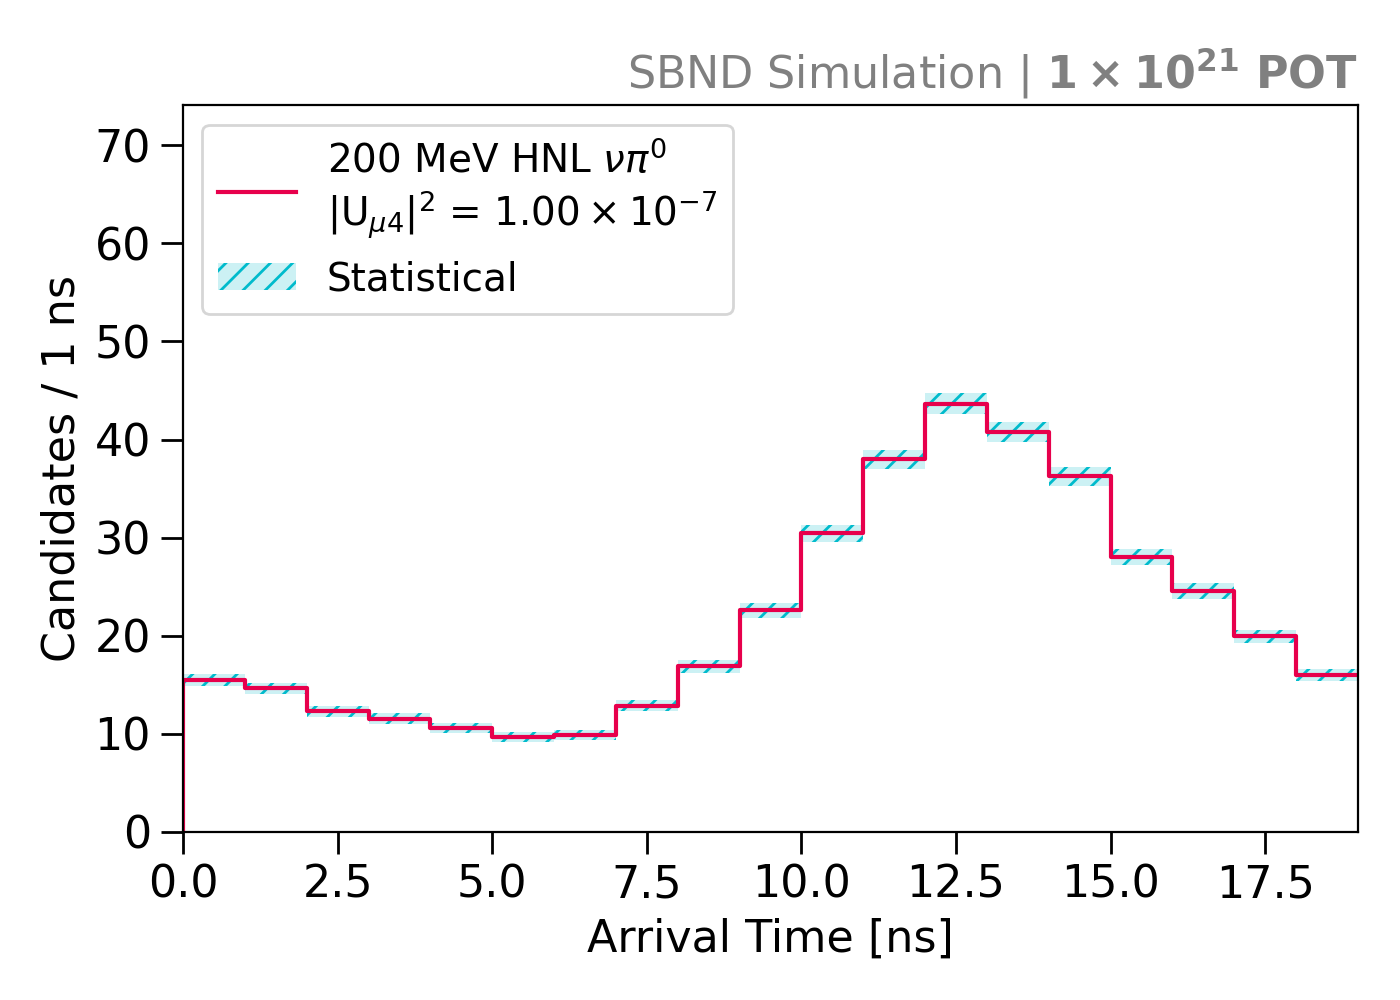
\includegraphics[width=\textwidth]{hnl_statistics_error}
            \caption{Statistical}%
            \label{fig:hnl_stat}
        \end{subfigure}
        \hfill
        \begin{subfigure}[b]{0.495\textwidth}   
            \centering 
            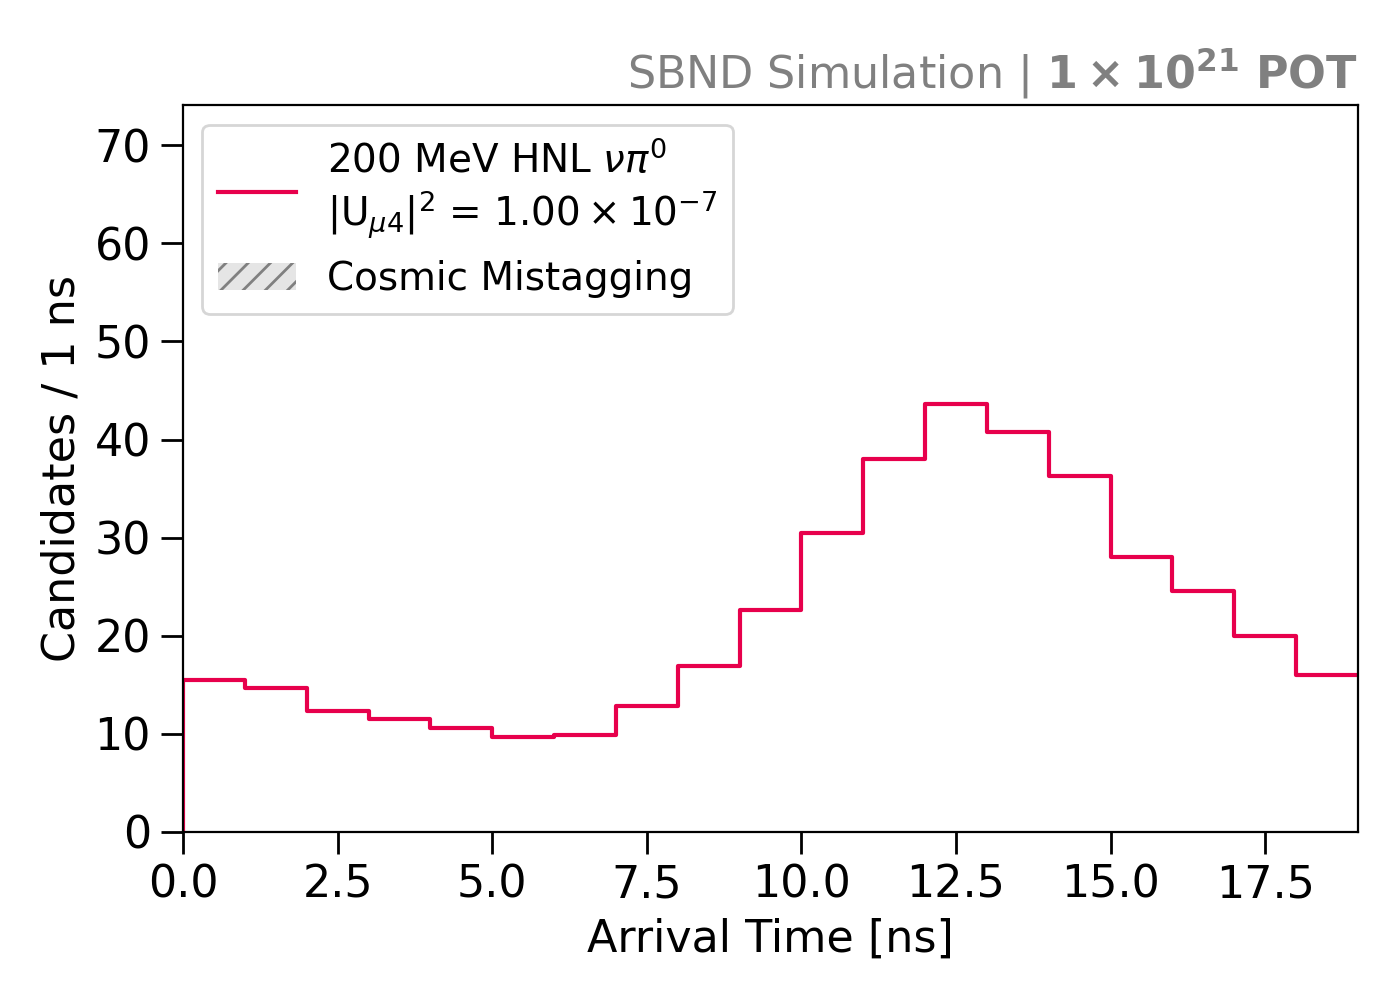
\includegraphics[width=\textwidth]{hnl_mistagging_error}
            \caption{Cosmic Mistagging}%
            \label{fig:hnl_mistag}
        \end{subfigure}
        \centering
        \begin{subfigure}[b]{0.495\textwidth}   
            \centering 
            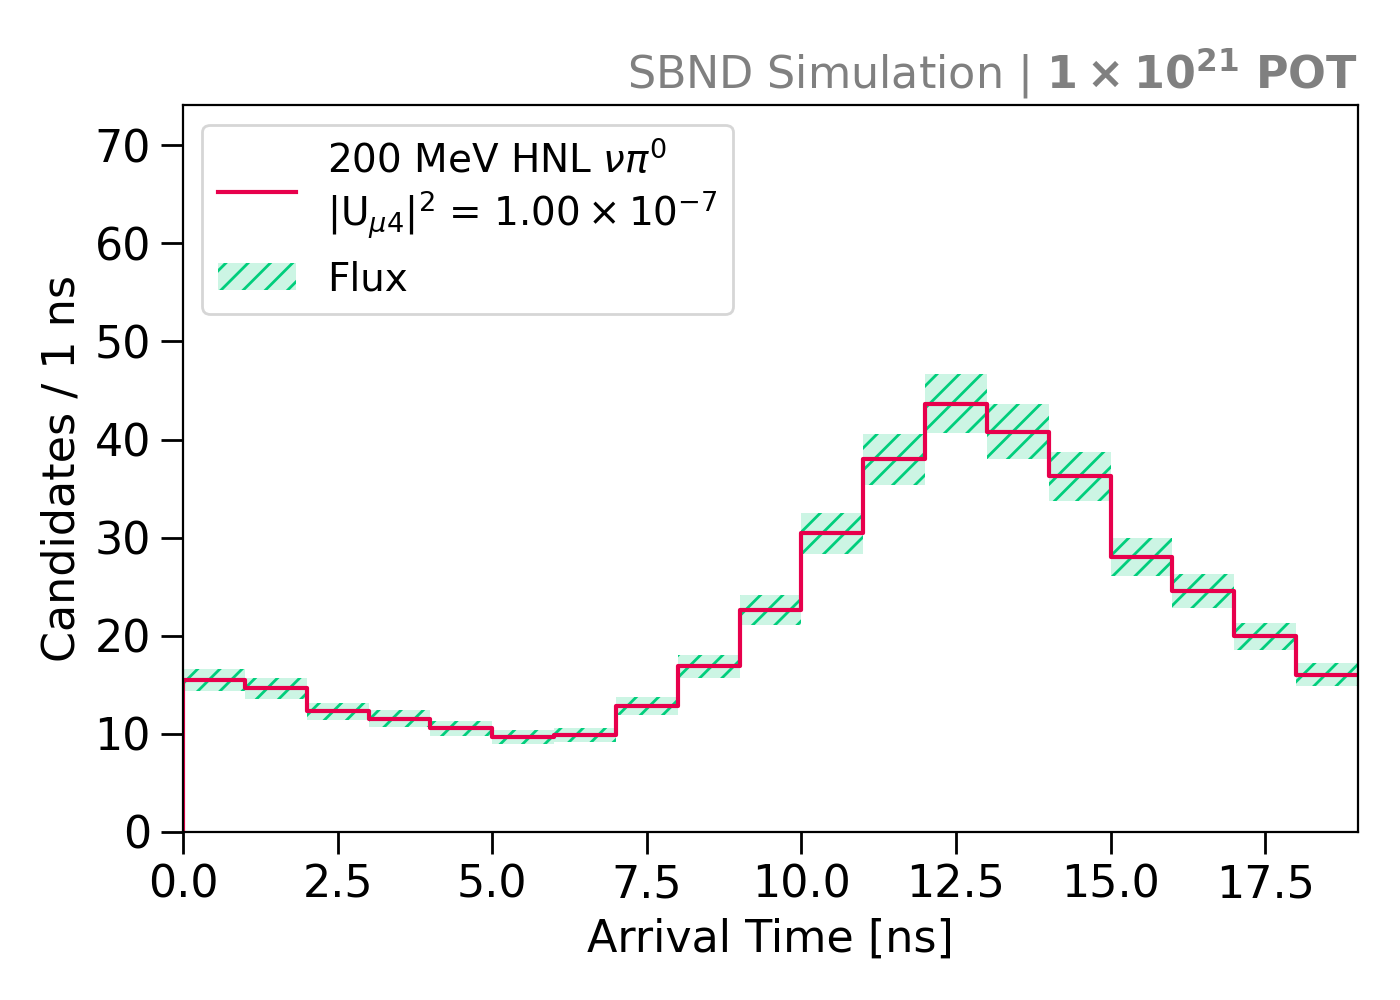
\includegraphics[width=\textwidth]{hnl_flux_error}
            \caption{Flux}%
            \label{fig:hnl_flux}
        \end{subfigure}
        \caption{
	Uncertainty sources of HNLs, including (a) statistical, (b) cosmic mistagging and (c) flux.
	}
        \label{fig:hnl_error}
	\vspace{0.5cm}
%\end{figure}
%\begin{figure}[htbp!] 
\centering    
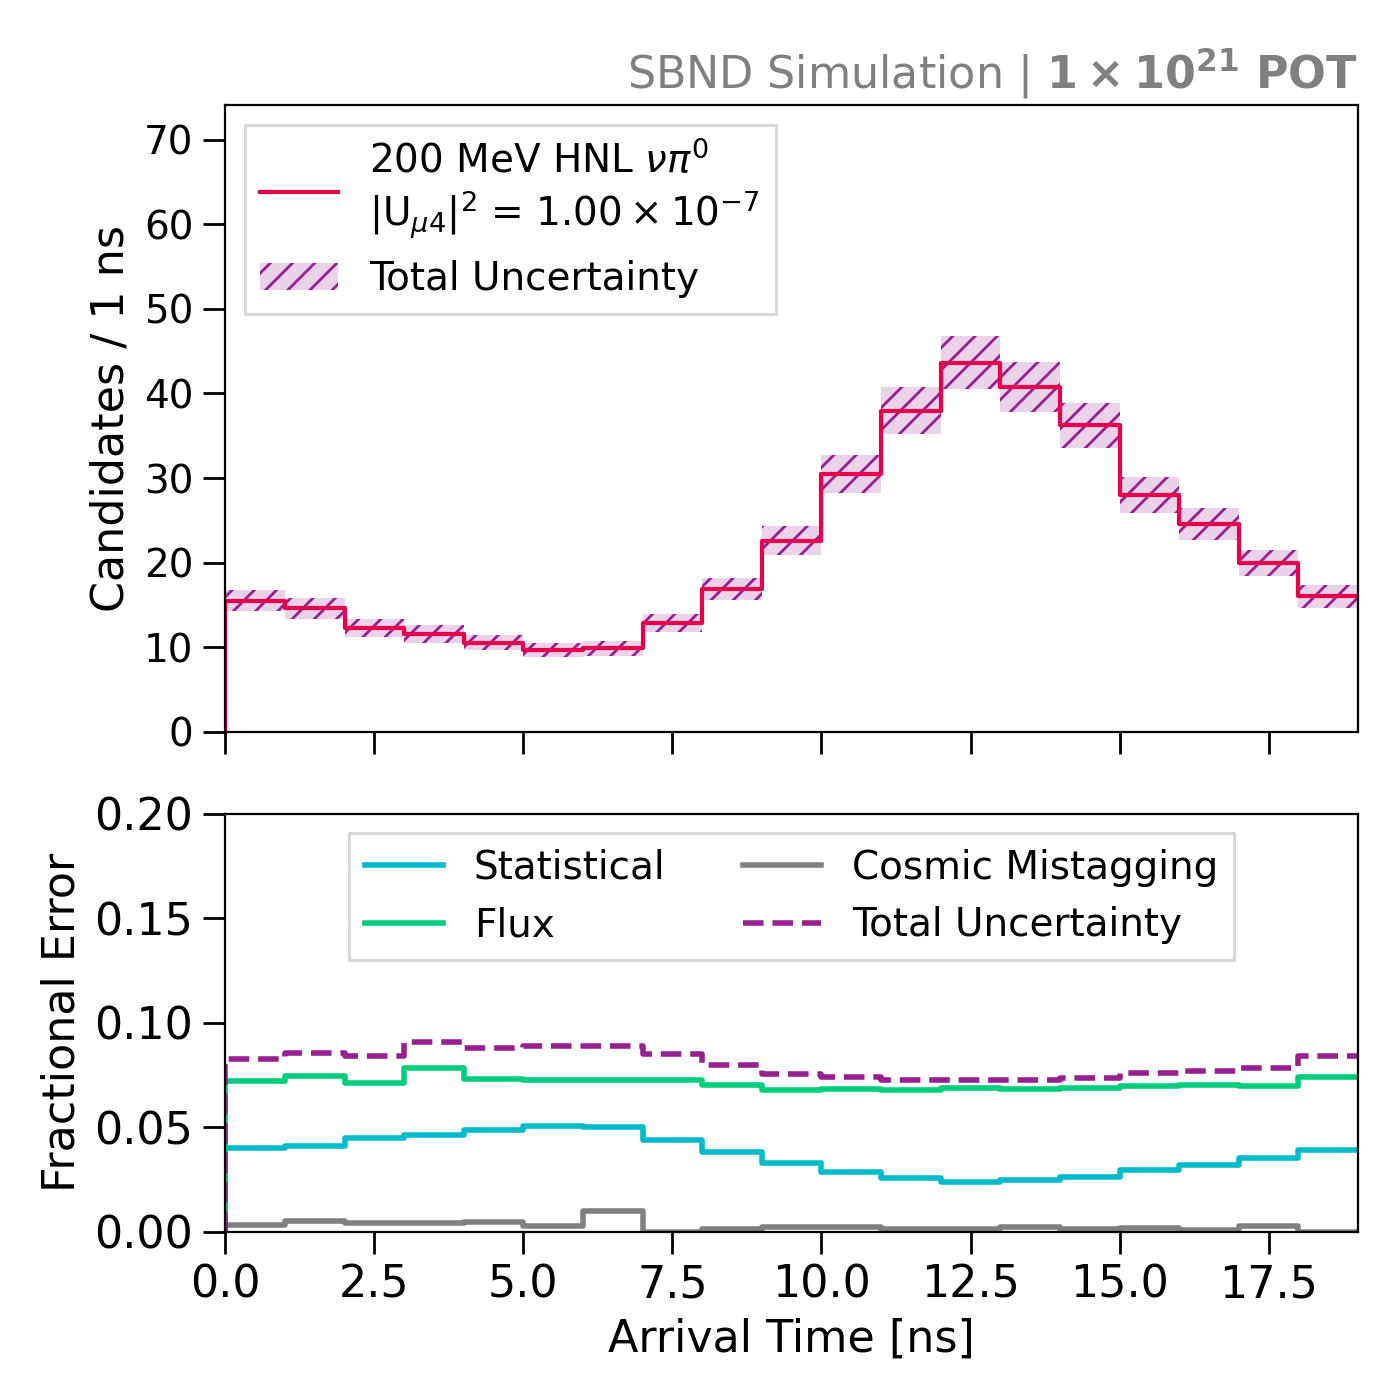
\includegraphics[width=0.5\textwidth]{hnl_error}
\caption[hnl error]{
Total uncertainty (top) and fractional uncertainties (bottom) of HNLs.
}
\label{fig:hnl_total_error}
\end{figure}

\subsection{Background Uncertainty Sources}
\label{sec:bkg_error}

For the background of SM neutrinos and cosmic muons, there are four primary sources of uncertainties: (1) statistical, (2) flux, (3) SM neutrino cross section and (4) detector.
The uncertainties due to statistics and flux are computed in the same manner as the uncertainty treatment of the HNL signal.
The detector systematic uncertainty is also currently not included but should be included in future work.
A new addition is the neutrino cross section uncertainty, of which the impact due to the cross section modelling 
is measured using the reweighting method.

The statistical uncertainty of the background was assessed using the number of SM neutrino and cosmic muon slices after the selection and computed using Eq. \ref{eq:stat_err}.
Fig. \ref{fig:bkg_stat} shows the statistical uncertainty of the background.
It is evident that the background statistics are abundant for bins at the centre of the beam bucket however, limited for bins at the edge.
Therefore, the statistical uncertainty is better constrained for bins at the centre, while bins at the edge have 
a higher statistical fluctuation.
This is visually evident in the statistical fractional uncertainty plotted in the blue line in the bottom figure of Fig. \ref{fig:bkg_total_error}.                                                                               
For bins at the centre of the beam bucket, the statistical fractional uncertainty is constrained at $< 20\%$ while.
For bins at the edge of the beam bucket distribution, particularly the first and last 4 bins, where the statistical fractional uncertainty reaches as high as $100\%$.

The flux systematic of the background was measured using the reweighting method similar to HNLs.              
One key difference in the flux systematics between the signal and the background is the uncertainties due to the secondary meson production in the BNB.                                                                           
Unlike HNLs coming from only $K^+$, SM neutrinos can result from $\pi^\pm$, $K^\pm$ and $K^0_L$ as previously plotted in Fig. \ref{fig:BNB_neutrino_flux}.
Particularly, the Sanford-Wang parametrisation for modelling the $\pi^+$ production introduces biases for NC $\pi^0$ interactions with energy < 300 MeV \cite{EdPhD}, which is the main background contributor.
Due to the selection requiring very high energetic showers, this bias is mitigated.
The resulting flux uncertainty of the background is plotted in Fig. \ref{fig:bkg_flux} and the flux fractional uncertainty is plotted in the green line in the bottom figure of Fig. \ref{fig:bkg_total_error}.
%TODO: check the percentage level
The flux fractional uncertainty is very well-constrained $<20 \%$ and consistent across the entire beam bucket distribution.

%TODO: add citation and add appendix
The SM neutrino cross section uncertainty was assessed using the SBN Event Weight, with systematic variable inputs from the GENIE generator.
There are two types of weights for SM neutrino interaction cross section: (1) weights associated with a group of correlated physics parameters and (2) weights associated with a single non-correlated physics parameter.
The SM neutrino systematics for a group of physics parameters are as follows
\begin{coloritemize}
\item\textbf{Charged Current Quasi-Elastic Scattering (CC-QE)}: Coefficients of the Z expansion of the axial form factor for CC-QE interactions are varied.
\item\textbf{Deep Inelastic Scattering (DIS)}: Parameters and correction factors of the Bodek-Yang model, which is used for modelling DIS cross sections, are varied. 
\item\textbf{Neutral Current Elastic Scattering (NC-EL)}: The axial mass and the strange axial vector of the dipole form factor of NC-EL interactions are varied.
\item\textbf{Neutral Current Resonant Scattering (NC-RES)}: The axial mass and the strange axial vector of the dipole form factor of NC-RES interactions are varied.
\item\textbf{Charged Current Resonant Scattering (CC-RES)}: The axial mass and the strange axial vector of the dipole form factor of CC-RES interactions are varied.
\item\textbf{Hadron Transport Interactions}: The mean free path, inelastic scattering, absorption, and pion production cross section are varied for both pions and nucleons.
\end{coloritemize}
The SM neutrino systematics for a single non-correlated physic parameter are as follows
\begin{coloritemize}
\item\textbf{Charged Current Quasi-Elastic Scattering (CC-QE)}: The shape of vector form factor, the random phase approximation and the strength of the Coulomb corrections of CC-QE interactions are varied.
\item\textbf{Meson Exchange Current Interactions (MEC)}: The decay angle and the normalisation factor of CC-MEC and NC-MEC are varied.
\item\textbf{Coherent Scattering (COH)}: Normalisation factors of NC-COH and CC-COH cross section interactions are varied.
\item\textbf{NonRES Backgrounds}: Non-resonant backgrounds are varied for CC and NC, $\nu$ and $\bar{\nu}$, neutron and proton, 1$\pi$ and 2$\pi$ for a total of 16 systematic parameters.
\item\textbf{Angular Distribution}: The angular distribution of $\gamma$ and $\pi$ are varied.
\item\textbf{Branching Fraction}: The branching fraction scale factor for resonant  decays with either a single $\gamma$ or $\pi$ are varied.
\end{coloritemize}
Fig. \ref{fig:bkg_xsec} shows the combined uncertainty of all the SM neutrino interaction cross section systematics.
Compared to statistical and flux uncertainties, the magnitude of the cross section uncertainty is significantly larger.
This is due to the primary background after selection being NC $\pi^0$, of which the cross section is not well-measured.  
Uncertainties associated with NC-COH and NC-RES scattering are the main contributors to this channel.
Moreover, a small fraction of CC $\nu_e$ interactions remains after selection and the cross section is also not well-measured.
For this channel, uncertainties associated with CC-QE scattering systematics contribute the most.
Finally, uncertainties for modelling hadron transport interactions and NonRES backgrounds of NC1$\pi$ interactions are significant contributors to the cross section uncertainty.

The cross section fractional uncertainty is plotted in the orange line in the bottom figure of Fig. \ref{fig:bkg_total_error}.
For bins at the centre of the beam bucket distribution, it is the lowest in the entire distribution at $< 50\%$.
It increases towards the bins at the edge of the beam bucket, reaching almost $100 \%$ for very low statistics bins.

The total fractional uncertainty combining the statistical, flux and cross section uncertainty, is plotted in the purple line.
For bins at the edge of the bucket, which are the bins driving the sensitivity limits, the total uncertainty is particularly high at $> 100\%$ due to the combined contribution from all three uncertainty sources.

%TODO: Update plots to after POT AND full background
\begin{figure}[htbp!]
        \begin{subfigure}[b]{0.495\textwidth}   
            \centering 
            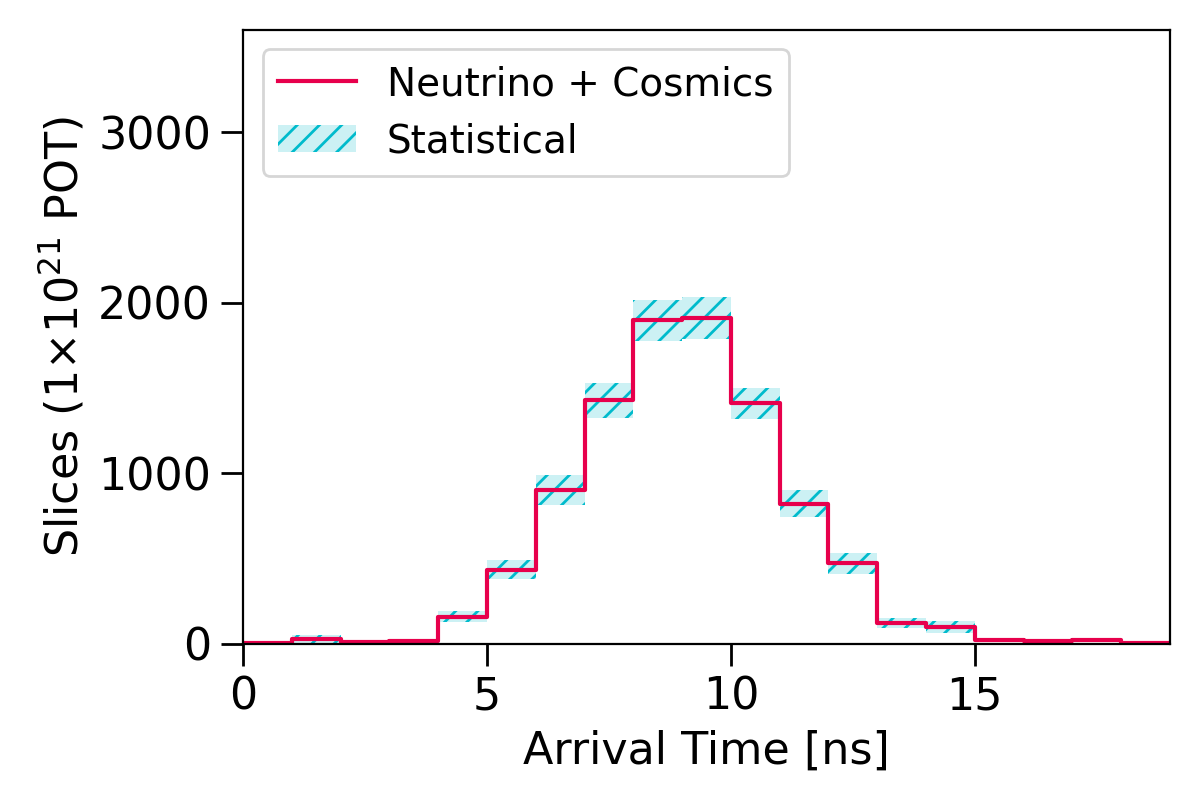
\includegraphics[width=\textwidth]{bkg_statistics_error}
            \caption{Statistical}%
            \label{fig:bkg_stat}
        \end{subfigure}
        \hfill
        \begin{subfigure}[b]{0.495\textwidth}   
            \centering 
            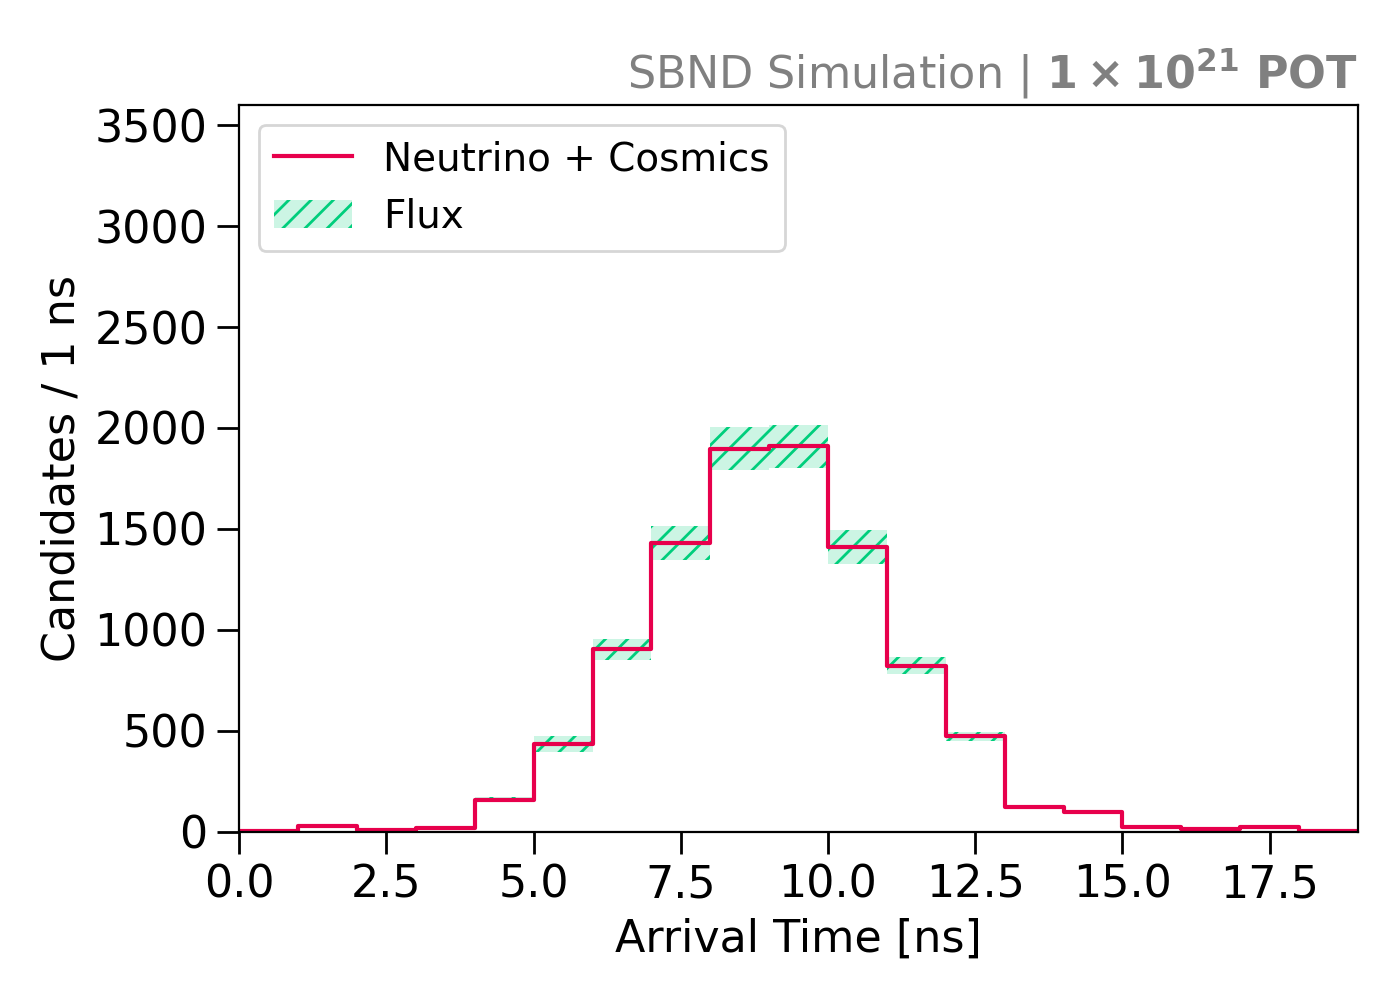
\includegraphics[width=\textwidth]{bkg_flx_error}
            \caption{Flux}%
            \label{fig:bkg_flux}
        \end{subfigure}
        \centering
        \begin{subfigure}[b]{0.495\textwidth}   
            \centering 
            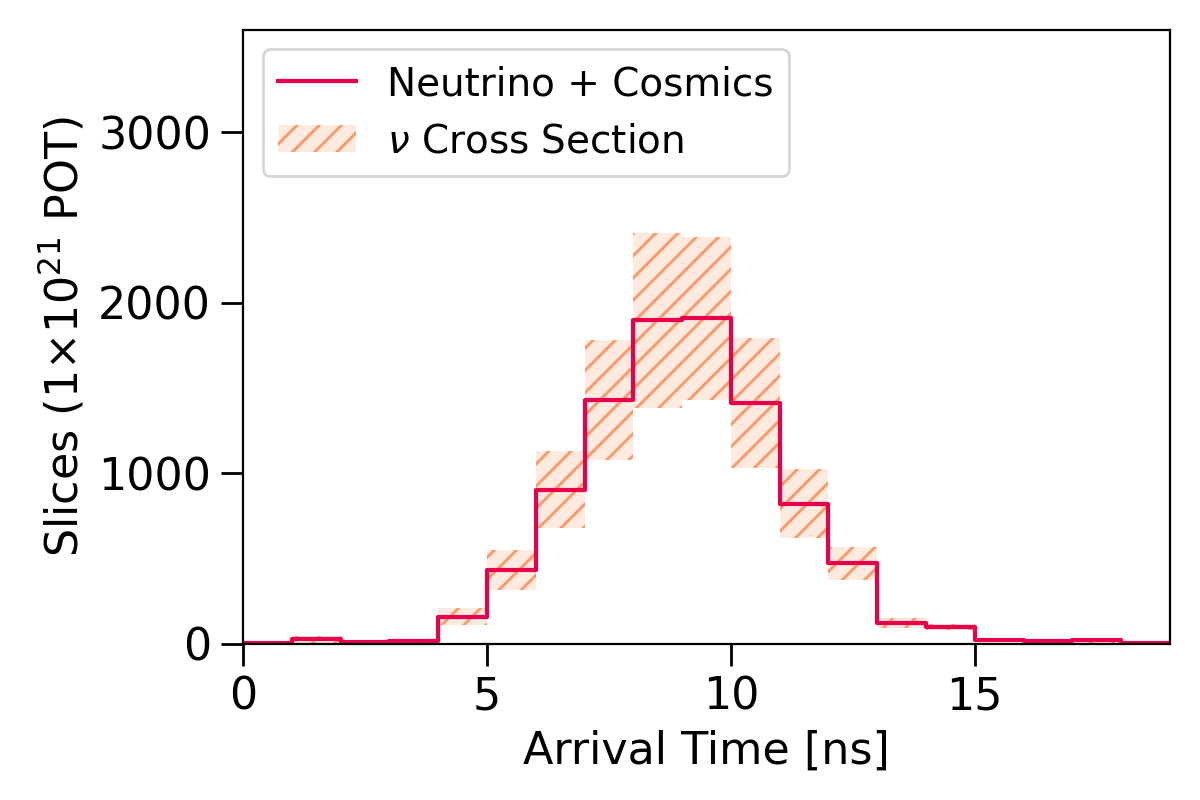
\includegraphics[width=\textwidth]{bkg_xsec_error}
            \caption{SM Neutrino Cross Section}%
            \label{fig:bkg_xsec}
        \end{subfigure}
        \caption{
	Uncertainty sources of SM neutrino and cosmic backgrounds, including (a) statistical, (b) flux and (c) SM neutrino cross section.
	}
        \label{fig:bkg_error}
	\vspace{0.5cm}
%\end{figure}
%\begin{figure}[htbp!] 
\centering    
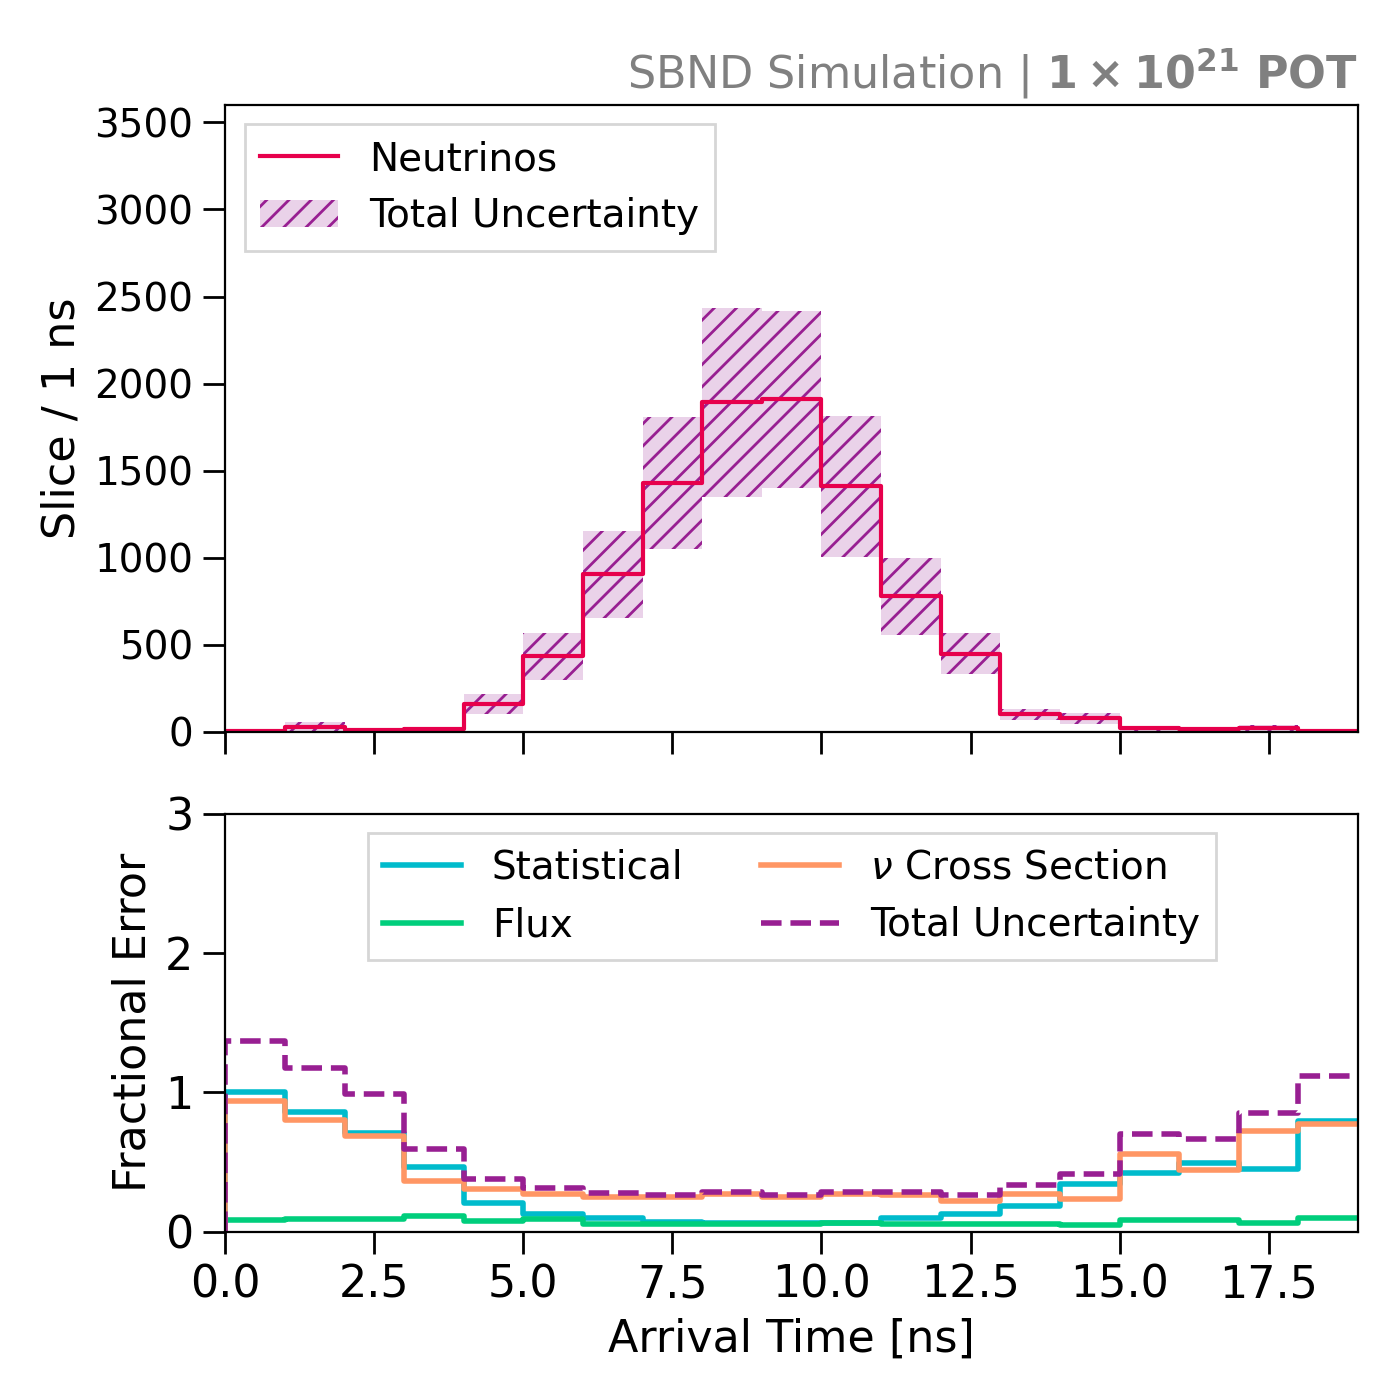
\includegraphics[width=0.5\textwidth]{bkg_error}
\caption[bkg error]{
Total uncertainty (top) and fractional uncertainties (bottom) of SM neutrino and cosmic backgrounds.
}
\label{fig:bkg_total_error}
\end{figure}
%********************************** %First Section  **************************************

\section{Limits Setting Procedure}
\label{sec:limit_procedure}

The limit setting procedure employs the likelihood-based hypothesis test \cite{asymptotic_test}, of which likelihood functions are constructed using the beam bucket distribution of signals and backgrounds.
The end-to-end procedure was performed using the \texttt{pyhf} package \cite{pyhf, pyhf_joss}.
This section begins with the definition of hypotheses for exclusion limits in Section \ref{sec:hypothesis_def} and the construction of the test statistic for each hypothesis in Section \ref{sec:llh_test}.
Then, the CL$_{s}$ method to determine \textit{p}-values of test statistics is described in Section \ref{sec:cls} and two approaches of computing test statistics are presented in Section \ref{sec:compute_test}. 
Finally, an overview of the limits setting done under the hood of the \texttt{pyhf} package is given in Section \ref{sec:set_limits} 

%This section will detail the hypothesis testing .

%Validation of the result acquired from the \textit{pyhf} package and the construction of likelihood functions using \textit{pyhf} are also presented.

%The test statistic is based on the likelihood ratio describing the probability of the observed data under the assumption of model parameters, allowing for the construction of the null and test hypotheses on the parameters.
%The resulting \textit{p}-values from the null and test hypotheses are then used to compute a modified $p$-value using the Confidence Levels (CL$_{s}$) method \cite{CLs_Junk, CLs_Read} to set the upper limits on the coupling $|U_{\mu4}|^{2}$. 

\subsection{Hypothesis Definition}
\label{sec:hypothesis_def}
The setting limit procedure employs the frequentist approach by performing hypothesis testing to quantify the level of agreement between the observed data and a given hypothesis $H$.
To exclude a signal region, the test hypothesis $H_{b}$ is defined as describing only known processes, or a background-only model.
Meanwhile, the null hypothesis $H_{s+b}$ is defined as the model including both background and signal processes.

A given hypothesis $H$ is constructed to represent the expectation value for an observable distribution, which is chosen to be the beam bucket distribution.
For a series of observations $n$, the expectation value of the $i$th bin can be constructed as 
\begin{equation}
    E[n_i] = \mu s_i + b_i    
\end{equation}
where $s_i$ and $b_i$ are the number of entries from the signal and background distributions for bin $i$.
The \textit{parameter of interest} $\mu$ determines the strength of the signal process, where $\mu = 0$ corresponds to the background-only $H_{b}$ hypothesis and $\mu = 1$ corresponds to the nominal signal $H_{s+b}$ hypothesis.
It is an unconstrained parameter and is written separately from other parameters in the hypothesis.
In the HNL search, varying the $\mu$ parameter is equivalent to varying the coupling $|U_{\mu4}|^{2}$.
Other parameters in the hypothesis characterising the shape of the distributions are grouped as \textit{nuisance parameters}, denoted as $\theta$.
Then, the null and test hypotheses can be formally written as
\begin{align}
    Null\ hypothesis:\ H_{s+b} = H (\mu = 1, \theta) \\
    Test\ hypothesis:\ H_{b} = H (\mu = 0, \theta)
\end{align}

\subsection{Likelihood-based Test Statistic}
\label{sec:llh_test}

To exclude the null hypothesis $H_{s+b}$ at some confidence levels, a test statistic is performed for a hypothesised $\mu$ against $H_{s+b}$ and $H_{b}$.
To construct a test statistic for a multi-binned histogram, likelihood-based functions are chosen.
The likelihood function is the product of Poisson probabilities of all bins in the histogram \cite{asymptotic_test}
\begin{equation}
\label{eq:LLH_func}
    %L(\mu, \boldsymbol{\theta}) =  \prod_{i=1}^{N} \frac{(\mu s_i + b_i)^{n_i}}{n_i!} e^{-(\mu s_i + b_i)}  \prod_{k=1}^{M} \frac{u_k^{m_k}}{m_k!}e^{-u_k}
    L(\mu, \theta) =  \prod_{i=1}^{N} \frac{(\mu s_i + b_i)^{n_i}}{n_i!} e^{-(\mu s_i + b_i)}  \prod_{\theta\in\theta} c_\theta(a_\theta|\theta)
\end{equation}
The first product describes the likelihood of the histogram $n$ with bin index $i$, which is constructed using the beam bucket distribution of HNLs as signals and SM neutrinos with cosmics as backgrounds. 
The second product is a constraint term $c_\theta(a_\theta|\theta)$ with measurement $a_\theta$ constraining the nuisance parameter $\theta$.
Individual constraint term is added for each uncertainty of signals and backgrounds respectively, as discussed in Section \ref{sec:uncertainty}. 

For a hypothesised value of $\mu$, the profile likelihood ratio can be constructed from the likelihood function as \cite{asymptotic_test}
\begin{equation}
\label{eq:likelihood_ratio}
    \lambda(\mu) = \frac{L(\mu, \hat{\hat{\theta}}(\mu))}{L(\hat{\mu},\hat{\theta})}
\end{equation}
The numerator is the \textit{conditional} maximised likelihood for the hypothesised value $\mu$ and $\hat{\hat{\theta}}(\mu)$ is a function of $\mu$.
The denominator is the \textit{unconditional} maximised likelihood, where $\hat{\mu}$ and $\hat{\theta} = \hat{\hat{\theta}}(\hat{\mu})$ are the best fit parameters to the observed data.

A modification in the likelihood ratio is required for cases where the signal process only increases the mean event rate, such that $\mu \geq 0$.
If the observed data results in the best fit $\hat{\mu} < 0$, then the best level of agreement between the data and the prediction is forced to occur at $\hat{\mu} = 0$.
This is equivalent to the late arrival of HNLs relative to the SM neutrino beam bucket, which can only increase the event rate for bins at the edge of the beam bucket.
The profile likelihood ratio is then modified as \cite{asymptotic_test}
\begin{equation}
    \Tilde{\lambda}(\mu) =
    \begin{cases}
        \frac{L(\mu, \hat{\hat{\theta}}(\mu) )}{L(0, \hat{\hat{\theta}} (0))}\ \ \ \hat{\mu} < 0 \\
        \frac{L(\mu, \hat{\hat{\theta}}(\mu) )}{L(\hat{\mu}, \hat{\theta})}\ \ \ \hat{\mu} \geq 0 \\
    \end{cases}
\end{equation}
where $\hat{\hat{\theta}} (0)$ is a function of $\mu = 0$. 

From the modified profile likelihood ratio, the test statistic for setting upper limits is \cite{asymptotic_test}
\begin{equation}
    \Tilde{q}_\mu = 
    \begin{cases}
        -2\ln\Tilde{\lambda}(\mu)\ \ \ \hat{\mu} \leq \mu 
        \\
        0\ \ \ \ \ \ \ \ \ \ \  \ \ \ \ \hat{\mu} > \mu
    \end{cases}
    = 
    \begin{cases}
        -2\ln\frac{L(\mu, \hat{\hat{\theta}}(\mu) )}{L(0, \hat{\hat{\theta}} (0))}\ \ \ \hat{\mu} < 0. \\
        -2\ln\frac{L(\mu, \hat{\hat{\theta}}(\mu) )}{L(\hat{\mu}, \hat{\theta})}\ \ \ 0 \leq \hat{\mu} \leq \mu, \\
        0\ \ \ \ \ \ \ \ \ \ \ \ \ \ \ \ \ \ \ \ \hat{\mu} > \mu
    \end{cases}
\end{equation}
In the region $\hat{\mu} > \mu$, equivalent to an upward fluctuation in the data compared to the prediction, the test statistic $\Tilde{q}_\mu$ is set to 0.
For setting an upper limit, this fluctuation does not represent less incompatibility and therefore is not taken into the rejection region of the test.
A larger value of $\Tilde{q}_\mu$ corresponds to an increasing disagreement between the data and the prediction for the hypothesised $\mu$.

The distribution $f(\Tilde{q}_{\mu}|\mu^{\prime})$ of a test statistic $\Tilde{q}_\mu$ can be interpreted as a PDF.
The subscript of $\Tilde{q}$ refers to the value of $\mu$ being tested in the numerator of the likelihood ratio in Eq. \ref{eq:likelihood_ratio}. 
The second argument $\mu^{\prime}$ refers to the value of $\mu$ being assumed in the denominator of Eq. \ref{eq:likelihood_ratio}.
%As previously defined, $\mu^\prime = \hat{\mu}$ is the value that best describes the observed data.
For setting an upper limit with hypotheses testing, the PDF of interest is $\Tilde{q}_{\mu}$ under the assumption of a different strength parameter $\mu^{\prime} \neq \mu$.
Therefore, the corresponding PDFs for a test signal strength $\mu$, under the assumption of the null hypothesis $H_{s+b}$ and the test hypothesis $H_b$, are respectively as 
\begin{align}
    f(\Tilde{q}_\mu | s + b ) &= f(\Tilde{q}_\mu | \mu^{\prime} = 1 ) \\
    f(\Tilde{q}_\mu | b ) &= f(\Tilde{q}_\mu | \mu^{\prime} = 0 )
\end{align}

\subsection{The CL$_{\mathrm{s}}$ Method}
\label{sec:cls}

To quantify the level of significance of a test statistic, a $p$-value is computed as an integration of the PDF $f(\Tilde{q}_{\mu}|\mu^{\prime})$ on either side of $\hat{q} = \Tilde{q}_{\mu}(\mu = \hat{\mu}) $ where $\hat{q}$ is the test statistic value for the observed data.
Typically, one might only consider the $p$-value resulting from the null hypothesis $H_{s+b}$, denoted as $p_{s+b}$, to exclude the null hypothesis.
This represents the probability of finding data more background-like under the assumption that the signal is true, also known as the probability of getting the type I error in hypothesis testing.
%If $p_{s+b} < \alpha$, the null $H_{s+b}$ hypothesis can be excluded with a confidence level of $1 - \alpha$.


%Typically, a right-sided integration represents the probability of finding data of equal or greater incompatibility with prediction under the assumption of $\mu^{\prime}$.

However, this approach does not factor in the probability of finding data under the assumption of the background-only hypothesis.
In scenarios where the test statistic is not sensitive to the prediction models, the PDFs of the $H_{s+b}$ and $H_b$ hypotheses would greatly overlap each other.
One might make the mistake of interpreting having observed data highly contaminated with background-like events as a statement on the nominal signal hypothesis \cite{CLs_Read}.
Therefore, a penalty for poor background modelling is necessary to account for how sensitive the test statistic is to the prediction model.

The CL$_s$ method is a modified frequentist method to compute a modified $p$-value.
This statistical method was developed specifically by particle physics experiments for the purpose of discovery as well as exclusion. This is a conservative approximation of the confidence level to account for poor background modelling and/or statistical fluctuations.
Using the CL$_{s}$ method, the \textit{p}-values for the hypotheses $H_{s+b}$ and $H_b$ are defined as follows \cite{asymptotic_test, CLs_Junk, CLs_Read}
\begin{align}
\label{eq:psb}
    p_{s+b} & = \int_{\hat{q}}^{\infty} f(\Tilde{q}_\mu|s+b) d\Tilde{q}_\mu \\
\label{eq:pb}
    p_{b} & = \int^{\hat{q}}_{-\infty} f(\Tilde{q}_\mu|b) d\Tilde{q}_\mu
\end{align}
$p_{s+b}$ represents the probability of finding data more background-like under the assumption of the signal+background hypothesis $H_{s+b}$.
$p_b$ represents the probability of finding data more signal-like under the assumption of the background-only hypothesis $H_b$.

The modified \textit{p}-value is then computed from the \textit{p}-value for each hypothesis as \cite{asymptotic_test, CLs_Junk, CLs_Read}
\begin{equation}
\label{eq:cls}
    CL_{s} = \frac{CL_{s+b}}{CL_b}= \frac{p_{s+b}}{1-p_b}
\end{equation}
Since $(1 - p_b)$ only varies between 0 and 1, the resulting CL$_s$ is always greater or equal to $p_{s+b}$.
Thus, the CL$_{s}$ is more conservative in quantifying the Confidence Level (C.L.) of hypothesis testing.
The threshold was chosen to be 0.1, such that CL$_{s} < (1 - 0.9)$, equivalent to setting an upper limit with a C.L. of 90\%.
This level was motivated in order to compare against existing experiment results. 

\subsection{Computing Test Statistic Distributions}
\label{sec:compute_test}

One way to obtain the PDF of $\Tilde{q}_\mu$ for a given hypothesis is by throwing toys (or pseudo-experiments) sampled from the observables $n$, with constrained nuisance parameters $\theta$. 
Each toy result represents a potential outcome of $\Tilde{q}_\mu$ and thus, the toy distribution represent the test statistic $\Tilde{q}_\mu$ distribution.
For a study using MC samples without having the observed data to determine $\hat{q}$, one can consider the distribution under the assumption of the background-only hypothesis $H_b$.
In this case, $\hat{q} = \hat{q}_{expected}$ represents the \textit{expectation} given the model prediction and is taken as the median of the $H_b$ test statistic distribution, equivalent to assuming the observed data is the same as the background-only prediction. 

Fig, \ref{fig:stat_toy} shows an example PDF of $\Tilde{q}_\mu$ for a test signal strength $\mu$ acquired from 4000 toys thrown.
The $\Tilde{q}_\mu$ PDF under the assumption of $H_{s+b}$ and $H_b$ is shown in green and yellow respectively.
The value $\hat{q}_{expected}$ is plotted as the dashed red line.
The area under the curve $f(\Tilde{q}_\mu | s + b )$ to the right of $\hat{q}_{expected}$ gives the median $p_{s+b}$ and the area under the curve $f(\Tilde{q}_\mu | b )$ to the left gives the median $p_{b}$.
The CL$_s$ value is then calculated to give the expected limit on the signal strength $\mu$. 
To identify which $\mu$ value results in CL$_s < 0.1$, a range of $\mu$ is considered until the desired value CL$_s$ is achieved.  
The test signal strength $\mu$ plotted here gives exactly CL$_s < 0.1$.
%Variations of 1 and 2 standard deviations from the expected CL$_s$ is then computed.
\begin{figure}[hp!] 
\centering    
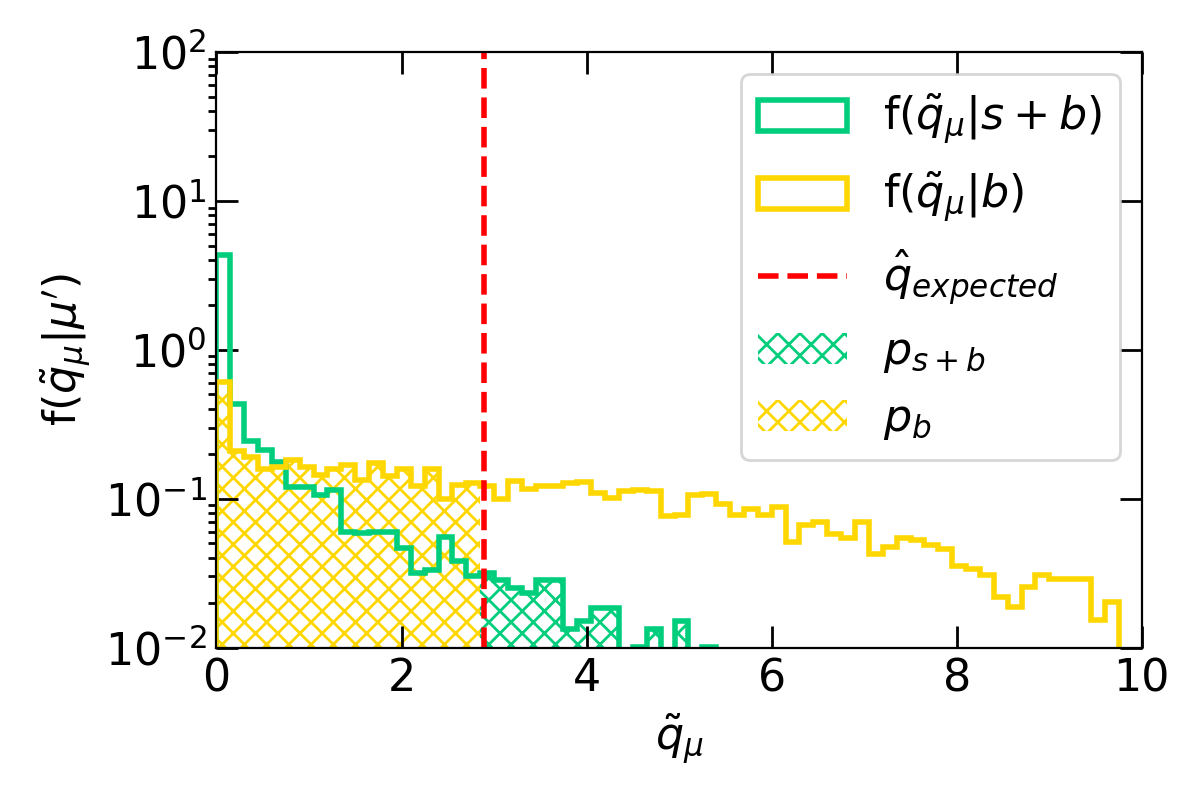
\includegraphics[width=0.65\textwidth]{toy}
\caption[stat toy]{Example of $\Tilde{q}_\mu$ distributions using the toy throwing approach.}
\label{fig:stat_toy}
\end{figure}

An alternative method to calculate the test statistic $\Tilde{q}_\mu$ and its PDF is by asymptotic approximation.
This approach assumes that $\hat{\mu}$ follows a Gaussian distribution around a mean of $\mu^{\prime}$ with a standard deviation of $\sigma$.
Via the \texttt{pyhf} package, PDFs are computed using the \texttt{HistFactory} module according to the formulae provided by Ref. \cite{asymptotic_test}.
Similar to the toy throwing approach for an MC study, $\hat{q}_{expected}$ is also taken as the median of the background-only $H_b$ test statistic distribution.
To determine CL$_s < 0.1$, \texttt{pyhf} scans over a range of $\mu$ and the best value is calculated using interpolation.

Fig. \ref{fig:stat_asymptotic} shows an example PDF of $\Tilde{q}_\mu$ computed using the asymptotic approximation.
The expected $\hat{q}_{expected}$ is plotted as the dashed red line. 
The median $p$-values under the $H_{s+b}$ and $H_b$ hypotheses are plotted as shaded green and yellow areas respectively.
The test signal strength $\mu$ shown here gives CL$_s < 0.1$.
Standard deviations of the CL$_s$ can also be computed by substituting $\mu^\prime$ with $\mu^{\prime} \pm N\sigma$, where $N\sigma$ is the number of standard deviations away from the mean $\mu^{\prime}$. 
A validation was also carried out to compare the signal strength $\mu$ resulting from the toy throwing and asymptotic approximation.
Both approaches returned $\mu$ values within 5\% of each other, showing a good agreement.

\begin{figure}[hp!] 
\centering    
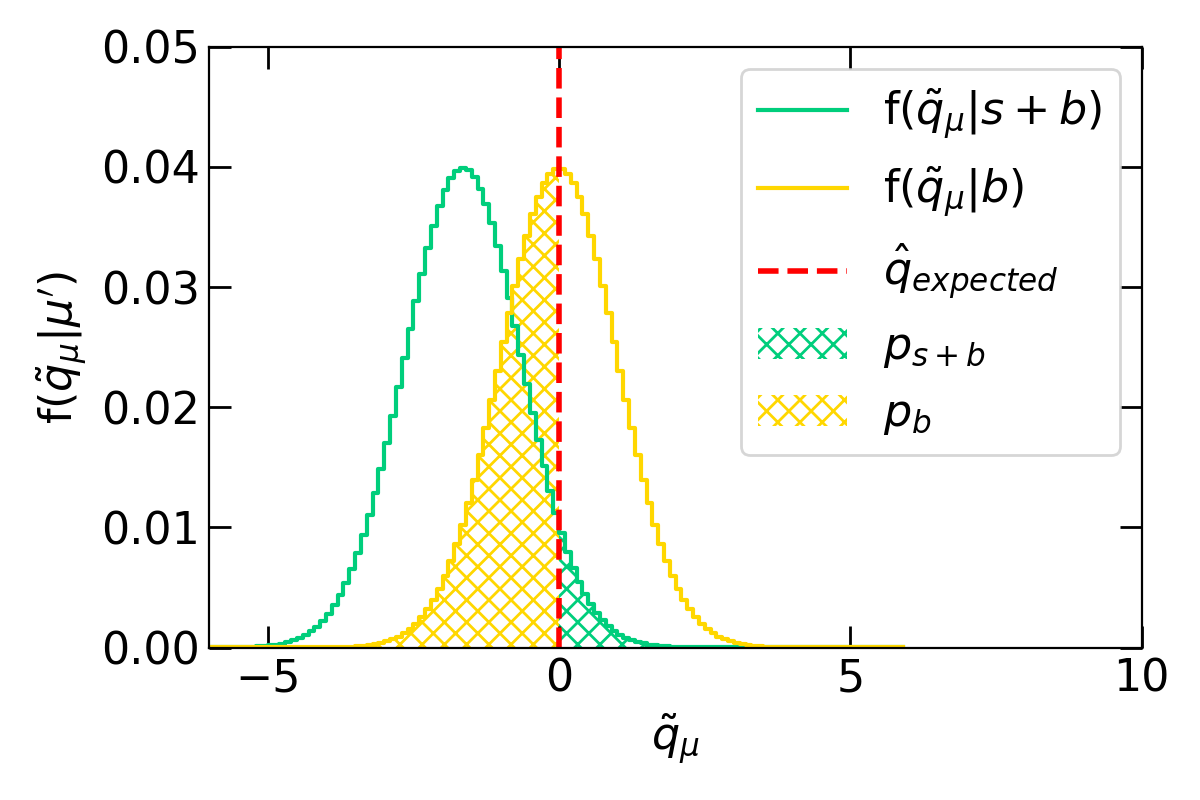
\includegraphics[width=0.65\textwidth]{asymtotic}
\caption[stat asymptotic]{Example of $\Tilde{q}_\mu$ distributions using the asymptotic approximation.}
\label{fig:stat_asymptotic}
\end{figure}

\subsection{Setting The Upper Limits}
\label{sec:set_limits}

The setting limit procedure is performed fully using the \texttt{pyhf} package, with the steps described in the previous section.
The beam bucket distribution is input into the \texttt{pyhf} package to infer the upper limit at C.L. of 90\%.
The histograms input to the background-only $H_{b}$ and the signal+background $H_{s+b}$ hypothesis are as following
\begin{itemize}
    \item $H_b$: The SM neutrinos and cosmic beam bucket distribution.
    \item $H_{s+b}$: The HNL beam bucket distribution on top of the background distribution. 
\end{itemize}

These histograms are the ingredients for the first product in Eq. \ref{eq:LLH_func}.
Since the likelihood functions are products of individual bins of the histograms, one can reduce the computing time by considering only high signal-to-noise bins that contribute the most to the sensitivity. 
As previously stated as the timing cut, the relevant high signal-to-noise bins are the first and last 4 bins of the beam bucket distribution, which lead to the same result as demonstrated later in Section \ref{sec:result}.

Three beam bucket distributions were used in the limit setting.
Appendix \ref{appendix_lenient} and \ref{appendix_stringent} contain the beam bucket distributions for signals and backgrounds after the lenient and stringent cut respectively, with all uncertainties propagated.
Additionally, appendix \ref{appendix_smeared} contains the smeared truth distributions under the assumption of timing reconstruction improvement as discussed in Section \ref{sec:truth_bucket}.
%, also used in the same limit setting.

The uncertainties of the beam bucket distribution discussed in Section \ref{sec:uncertainty} are the constraints on the nuisance parameters $c_\theta(a_\theta|\theta)$ in the second product Eq. \ref{eq:LLH_func}.
Different types of constraints can take different statistical shapes, which are called \textit{modifiers} in the \texttt{pyhf} package \cite{pyhf, pyhf_joss}.
Table \ref{table:constraint} summarises the uncertainties and their corresponding modifiers of the signal and background distribution.


For the signal distribution, the assumption is that the signal rate is relatively low and expected to follow a Poisson distribution.
Similarly, the cosmic mistagging rate falls under the same assumption since it is proportional to the signal rate. 
Thus, the modifier for both statistical and cosmic mistagging uncertainties of the signal distribution follows a Poisson shape, treating each bin uncorrelated. 
The flux uncertainty of the signal distribution uses a Gaussian-shaped modifier instead, to enable correlation bin-wise.

For the background distribution, the treatment of statistical uncertainty employs a modified version of the Beeston-Barlow method \cite{BeestonBarlow} to account for statistical fluctuations due to finite statistics.
The modifier in this case follows a Gaussian shape for bins with high statistics and falls back to a Poisson shape for bins with low statistics while treating each bin uncorrelated.                                            
Moreover, the flux and SM neutrino cross section uncertainty also use a Gaussian-shapred modifier, however, with correlation bin-by-bin.

\begin{table}[htbp!]
\begin{center}
\begin{tabular}{|c| c | c | c | c |} 
\hline 
& \textbf{Uncertainty} & \textbf{Modifier} & \textbf{Sample Correlation} & \textbf{Bin Correlation}\\
\hline &&&&\\[0.1cm]

\multirow{3}{*}{\rotatebox[origin=c]{90}{\parbox[c]{1.85cm}{\centering \textbf{Signal} }}} 

& Statistical & \multicolumn{1}{c|}{Poisson} & \multicolumn{1}{c|}{False} & \multicolumn{1}{c|}{False} \\ [1ex]

& Cosmic mis-tagging & \multicolumn{1}{c|}{Poisson} & \multicolumn{1}{c|}{False} & \multicolumn{1}{c|}{False} \\ [1ex]

& Flux & \multicolumn{1}{c|}{Gaussian} & \multicolumn{1}{c|}{False} & \multicolumn{1}{c|}{True} \\ [1ex]

\hline &&&&\\[0.1cm]

\multirow{3}{*}{\rotatebox[origin=c]{90}{\parbox[c]{1.85cm}{\centering \textbf{Background} }}} 

& Statistical & \multicolumn{1}{c|}{Gaussian} & \multicolumn{1}{c|}{False} & \multicolumn{1}{c|}{False} \\ [1ex]

& Flux & \multicolumn{1}{c|}{Gaussian} & \multicolumn{1}{c|}{False} & \multicolumn{1}{c|}{True} \\ [1ex]

& SM Neutrino Cross Section & \multicolumn{1}{c|}{Gaussian} & \multicolumn{1}{c|}{False} & \multicolumn{1}{c|}{True} \\ [1ex]
\hline
\end{tabular}
\end{center}
\caption{Table summarising modifiers used to constrain uncertainties.}
\label{table:constraint}
\end{table}

For a single mass point, \texttt{pyhf} performs a scanning of signal strength $\mu$ until the desired value giving the 90\% CL is determined. 
To infer from the signal strength $\mu$ to the coupling $|U_{\mu4}|^{2}$, the proportionality of the  number of signals  $N_{HNL}$ to the coupling is employed.
The signal rate observed at the detector is proportional to the coupling at the HNL production as well as the coupling at the HNL decay, and thus, $N_{HNL} \propto |U_{\mu4}|^{4}$.
The upper limit of the coupling is then $\sqrt{\mu}$ multiplied by the input coupling $|U_{\mu4}|^{2}$.
This process is repeated across all the mass points.
%********************************** %First Section  **************************************

\section{Results}
\label{sec:result}

Results acquired from three different beam bucket distributions are presented in this section.
The first two distributions were acquired by using fully reconstructed MC samples mimicking data, of which one 
was applied with a lenient selection as shown in Fig. \ref{fig:final_relaxed} and the other one was applied with a stringent selection as shown in Fig. \ref{fig:final_strict}.
The third distribution is the smeared truth as shown in Fig. \ref{fig:final_truth}, which was constructed by smearing \textit{true} variables without any detection simulation and reconstruction applied.
The smeared truth distribution was motivated under the assumption of a better timing reconstruction resolving the beam bucket with a resolution of 1.73 ns.
Unlike, the reconstructed distributions with full uncertainties propagated, the smeared truth distribution does not contain any uncertainties for simplification. 
Moreover, the first and last 4 bins of every distribution are also shown to demonstrate the significantly high signal-to-background ratio of these bins.

\begin{figure}[htbp!]
        \begin{subfigure}[b]{1.0\textwidth}
            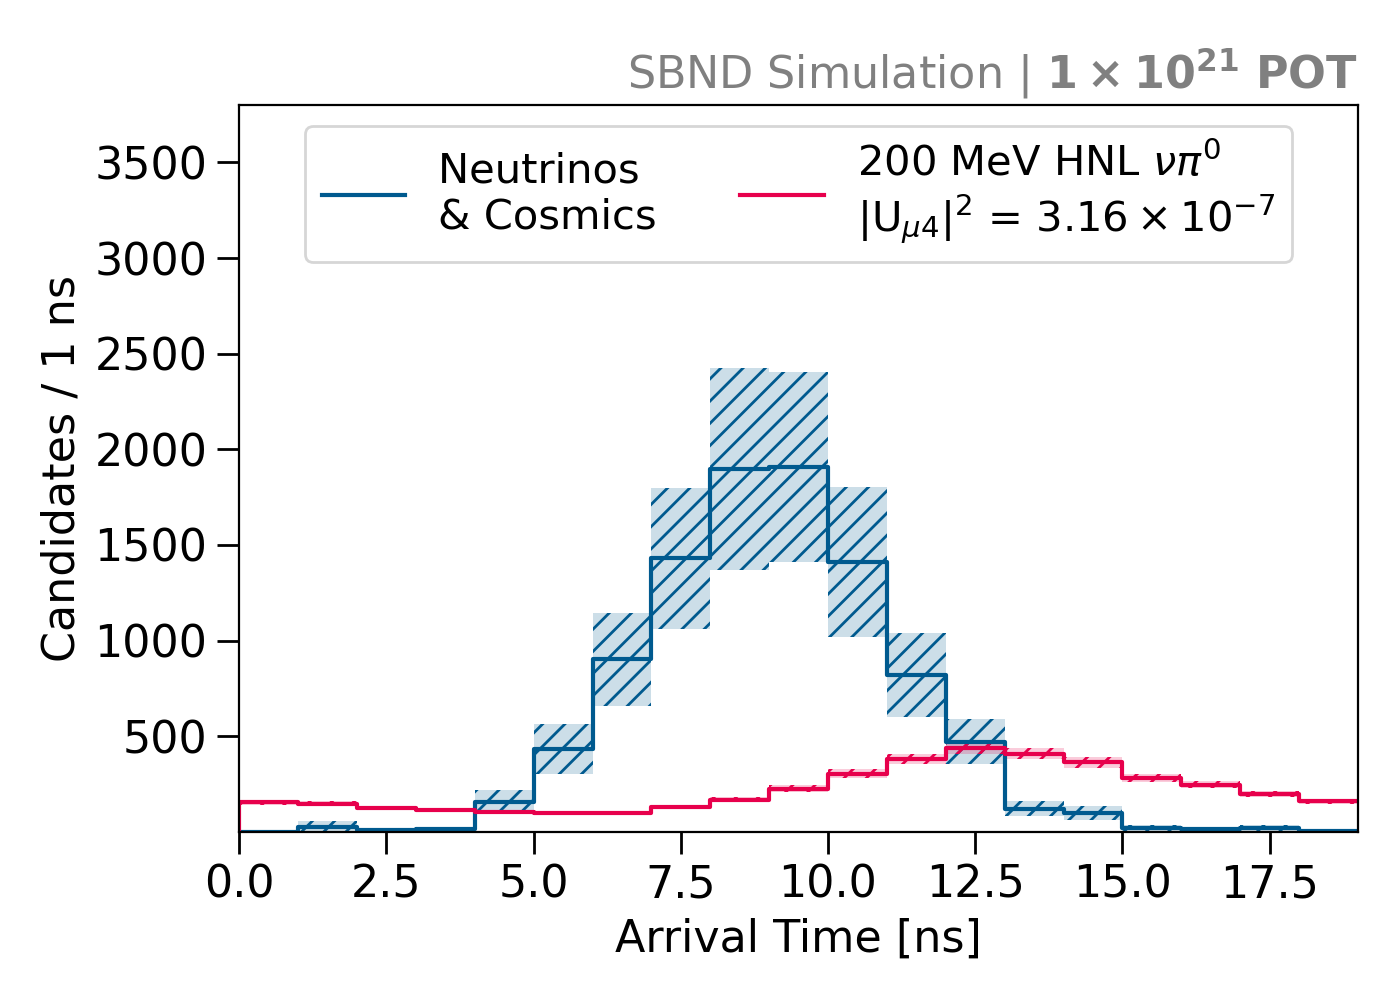
\includegraphics[width=0.5\textwidth]{relaxed_cut}
            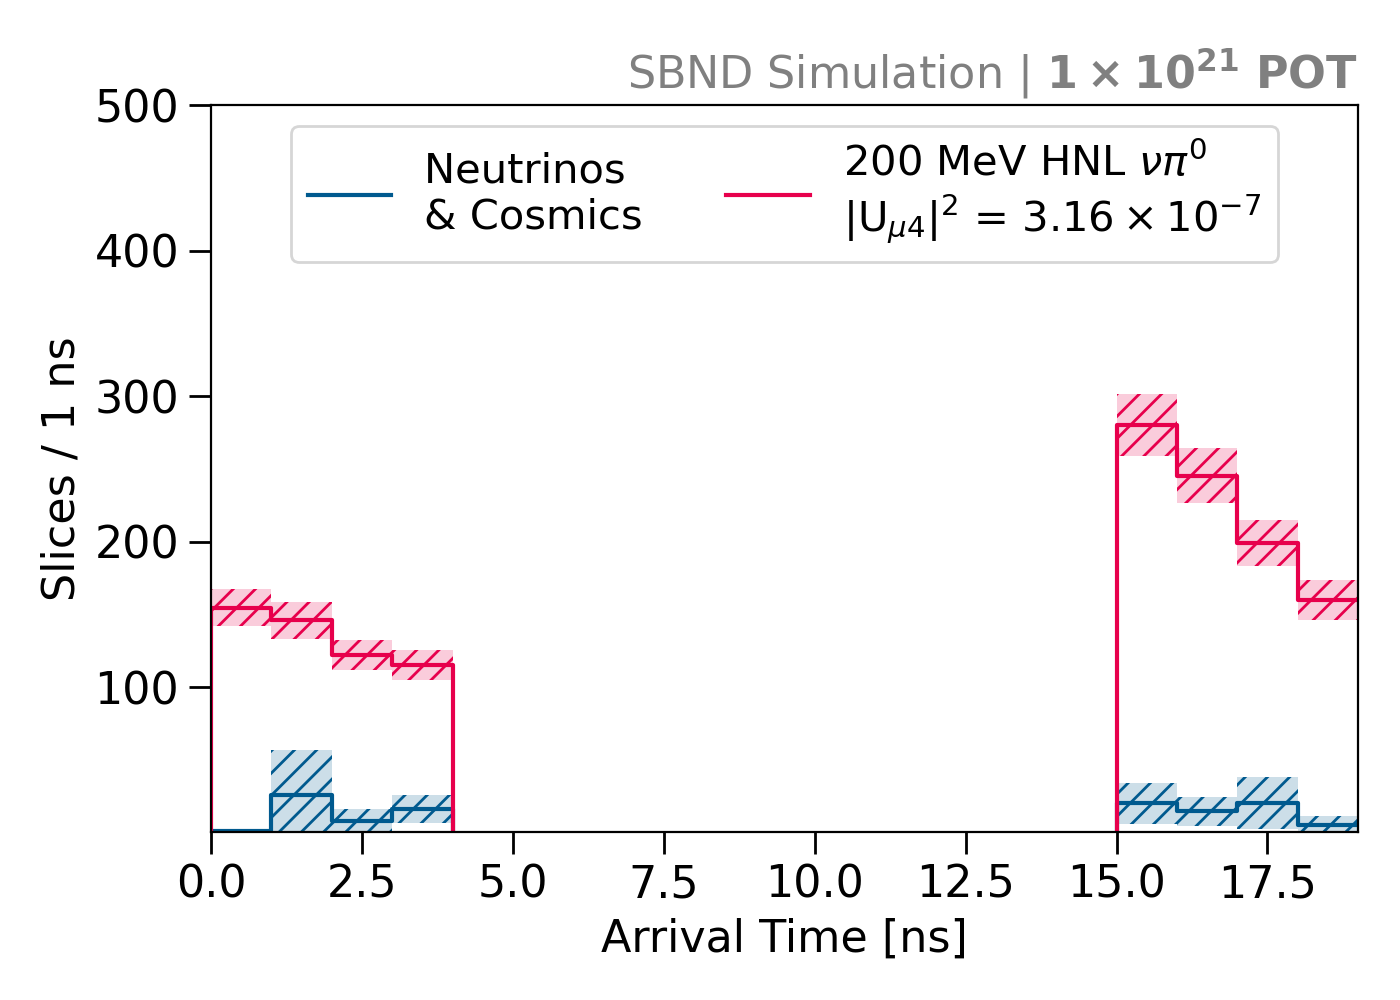
\includegraphics[width=0.5\textwidth]{relaxed_cut_edge}
            \caption{The lenient distribution}%
	    \label{fig:final_relaxed}
     	    \vspace{0.5cm}
        \end{subfigure}
        \begin{subfigure}[b]{1.0\textwidth}
            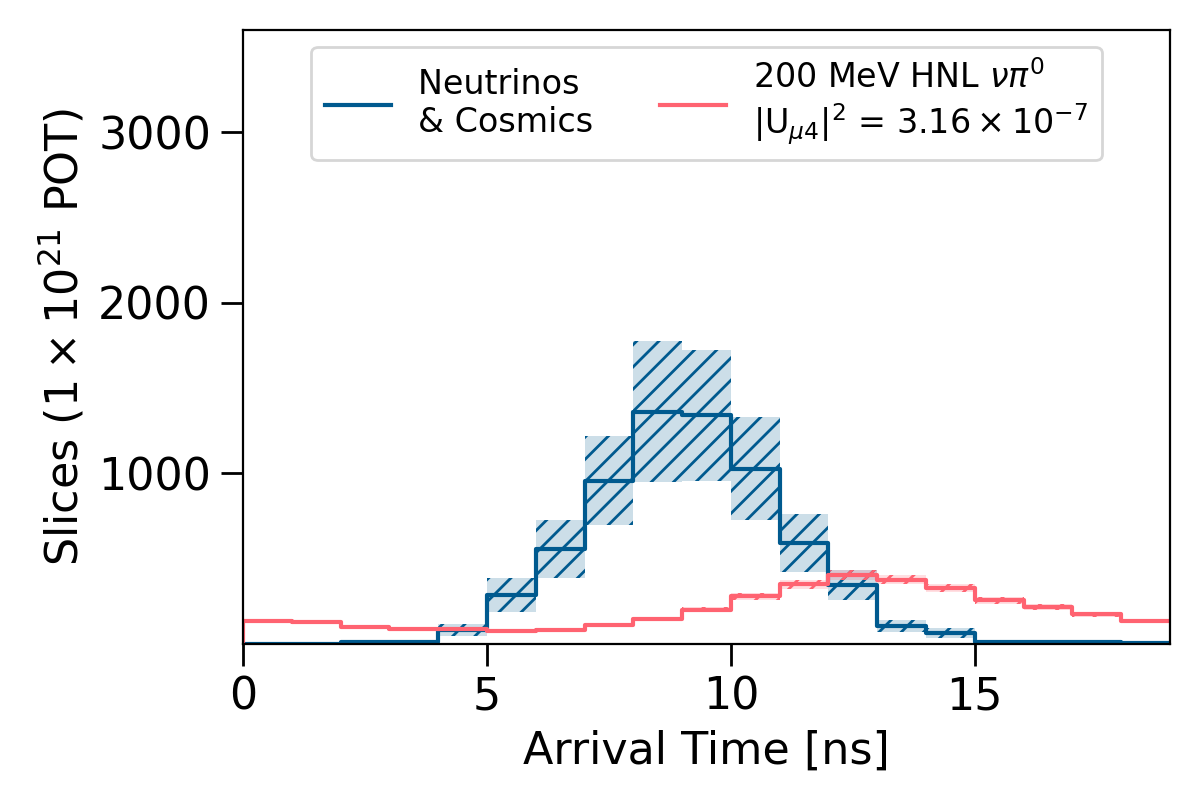
\includegraphics[width=0.5\textwidth]{strict_cut}
            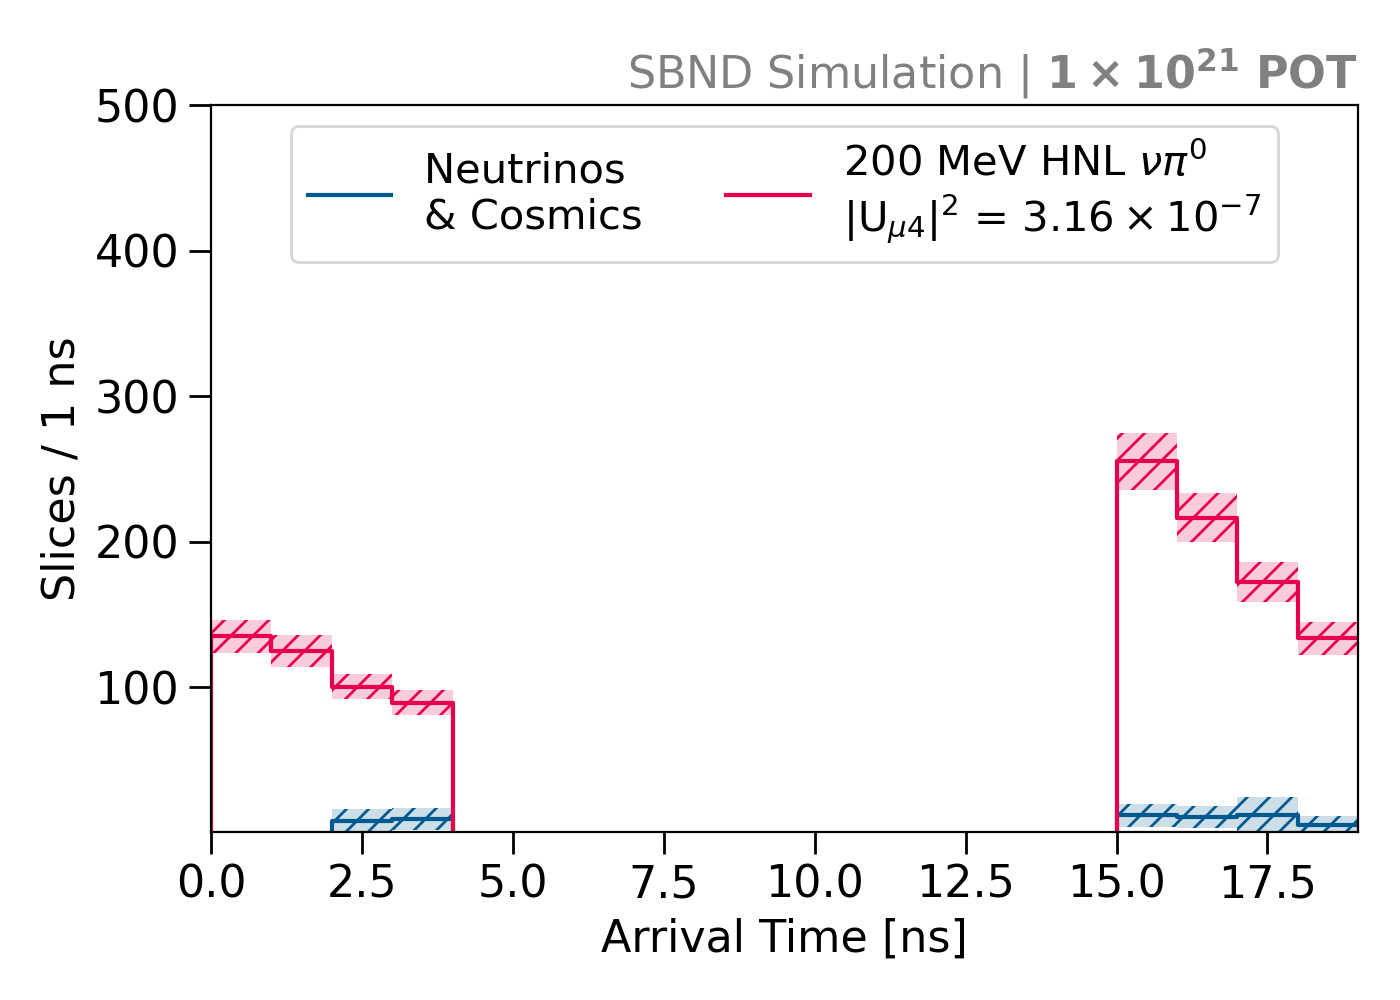
\includegraphics[width=0.5\textwidth]{strict_cut_edge}
            \caption{The stringent distribution}%
	    \label{fig:final_strict}
       	    \vspace{0.5cm}
        \end{subfigure}
        \begin{subfigure}[b]{1.0\textwidth}
            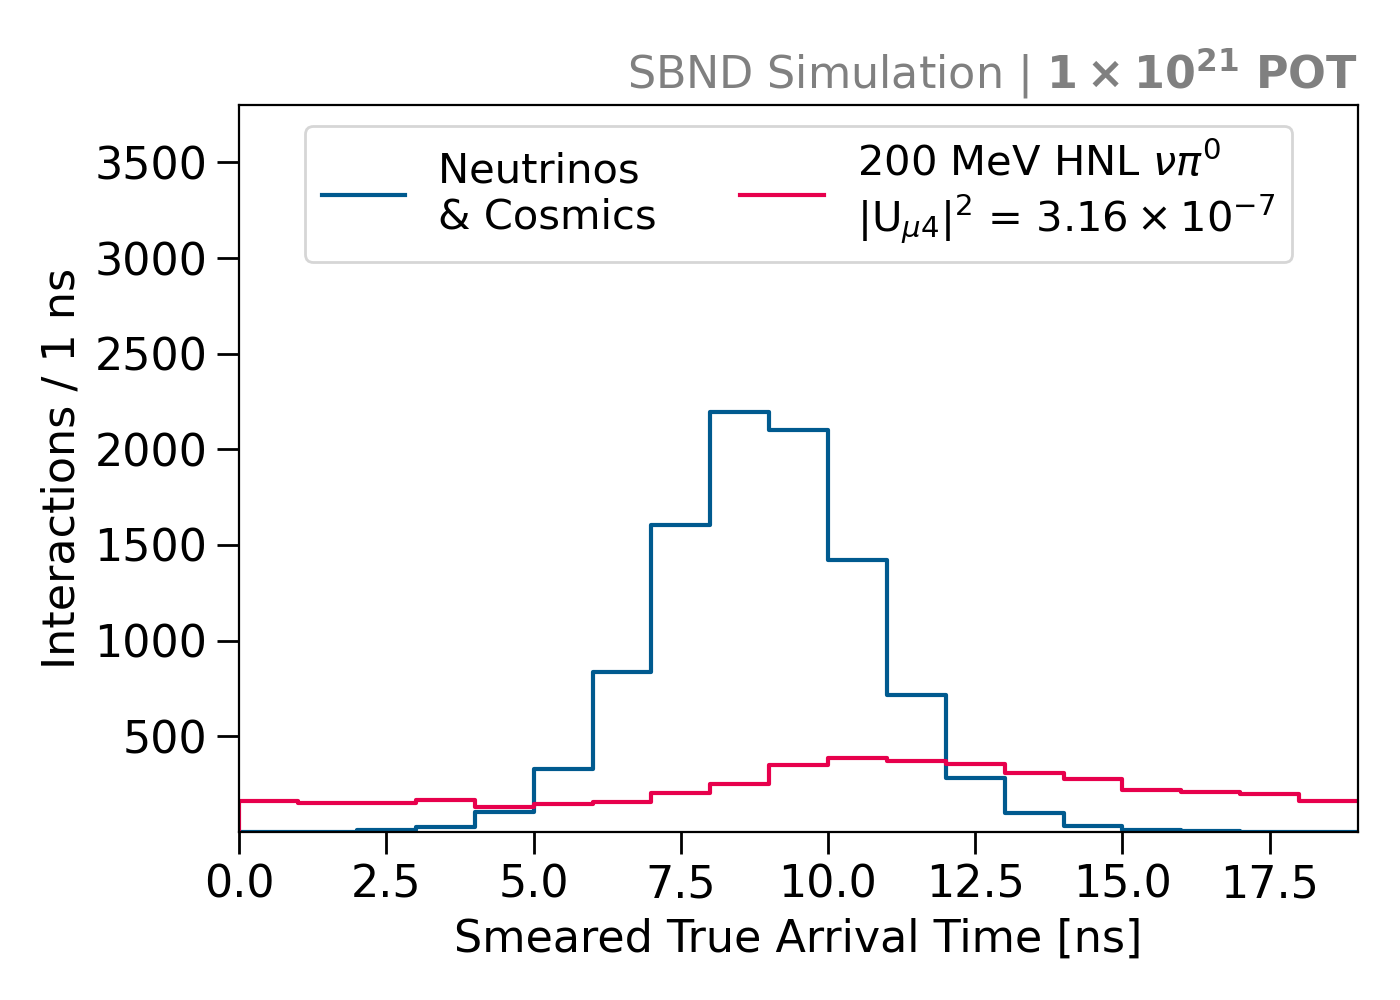
\includegraphics[width=0.5\textwidth]{smeared_truth}
            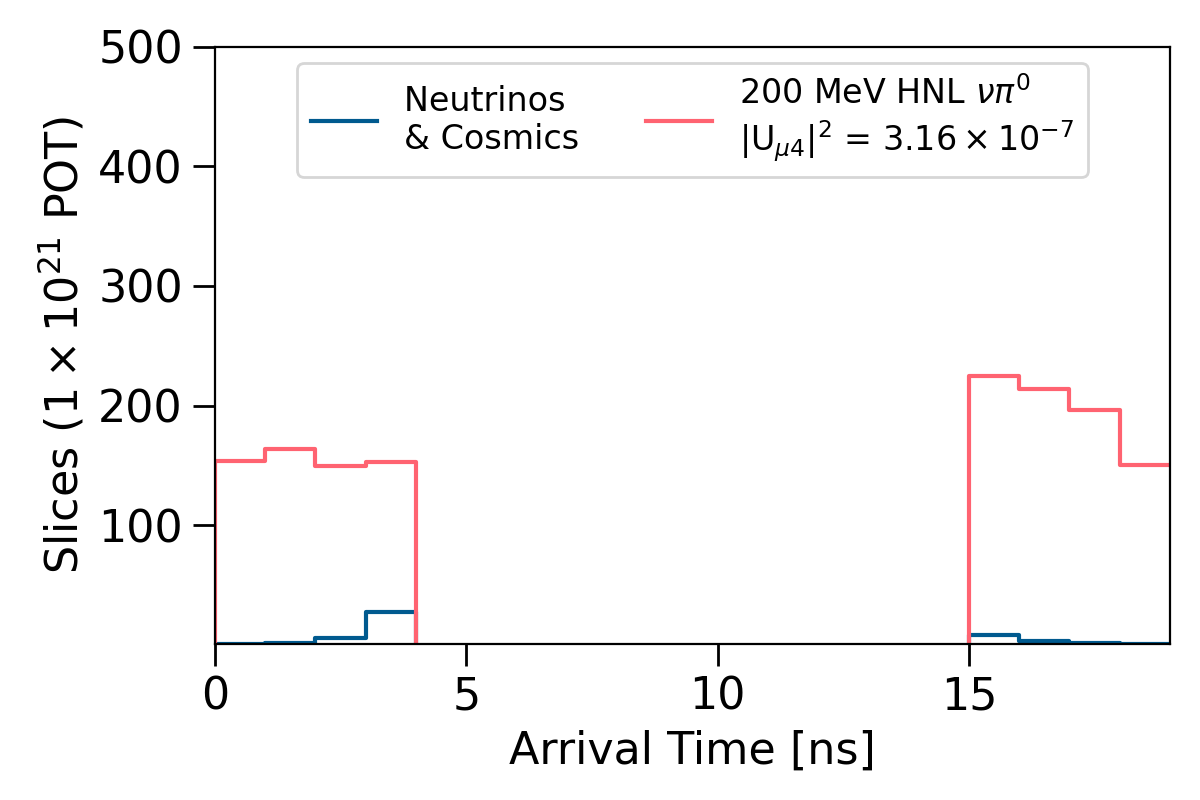
\includegraphics[width=0.5\textwidth]{smeared_truth_edge}
            \caption{The smeared truth distribution}%
	    \label{fig:final_truth}
     	    \vspace{0.5cm}
        \end{subfigure}
        \caption{
	Beam bucket distributions used for the limits setting, including (a) the lenient, (b) the stringent and (c) the smeared truth distribution.
	}
\end{figure}

\subsection{Comparison Across Different Beam Bucket Distributions}

The upper limits on the coupling of Majorana HNLs at 90\% C.L. are presented in Fig. \ref{fig:nupi0_reco_result}, comparing results from fitting the beam bucket distribution with the lenient and stringent distribution.
The expected limit is plotted as the solid black line.
The deviation band at 1 and 2$\sigma$ away from the expectation, also known as the \textit{Brazil} band, is plotted in shaded green and yellow respectively.
The lenient distribution results in a limit excluding the coupling $|U_{\mu4}|^2$ from $9.18 \times 10^{-7}$ to $1.35 \times 10^{-8}$ across the mass range from 140 to 260 MeV.
The stringent cut results in a more competitive limit, pushing the exclusion region of the coupling further down from $5.37 \times 10^{-7}$ to $7.65 \times 10^{-9}$ at the same mass range.
This is due to the stringent distribution having a better signal-to-background ratio for bins at the edge of the beam bucket.
This is evident when comparing between Fig. \ref{fig:final_relaxed} and \ref{fig:final_strict}, where the signal rate is very similar across the two distributions but the background rate is much lower in the stringent than the lenient distribution.
Particularly, the first two bins of the stringent distribution are background-free, thus, driving the limit significantly.

However, the magnitude of the Brazil band of the stringent result is larger than the lenient result, indicating that the stringent result has larger uncertainties.
This is likely due to the limited statistics of the background MC samples after the stringent selection.
As can be observed from bins at the edge of the beam bucket distribution shown in Fig. \ref{fig:final_strict}, the lack of background statistics might be insufficient to describe the underlying distribution, which can lead to large statistical fluctuations.                                  
Although the stringent distribution leads to a more competitive result, a future iteration of this selection is recommended to perform on larger statistics MC samples so that the statistical uncertainty can be better constrained.

\begin{figure}[b!]
    \centering
    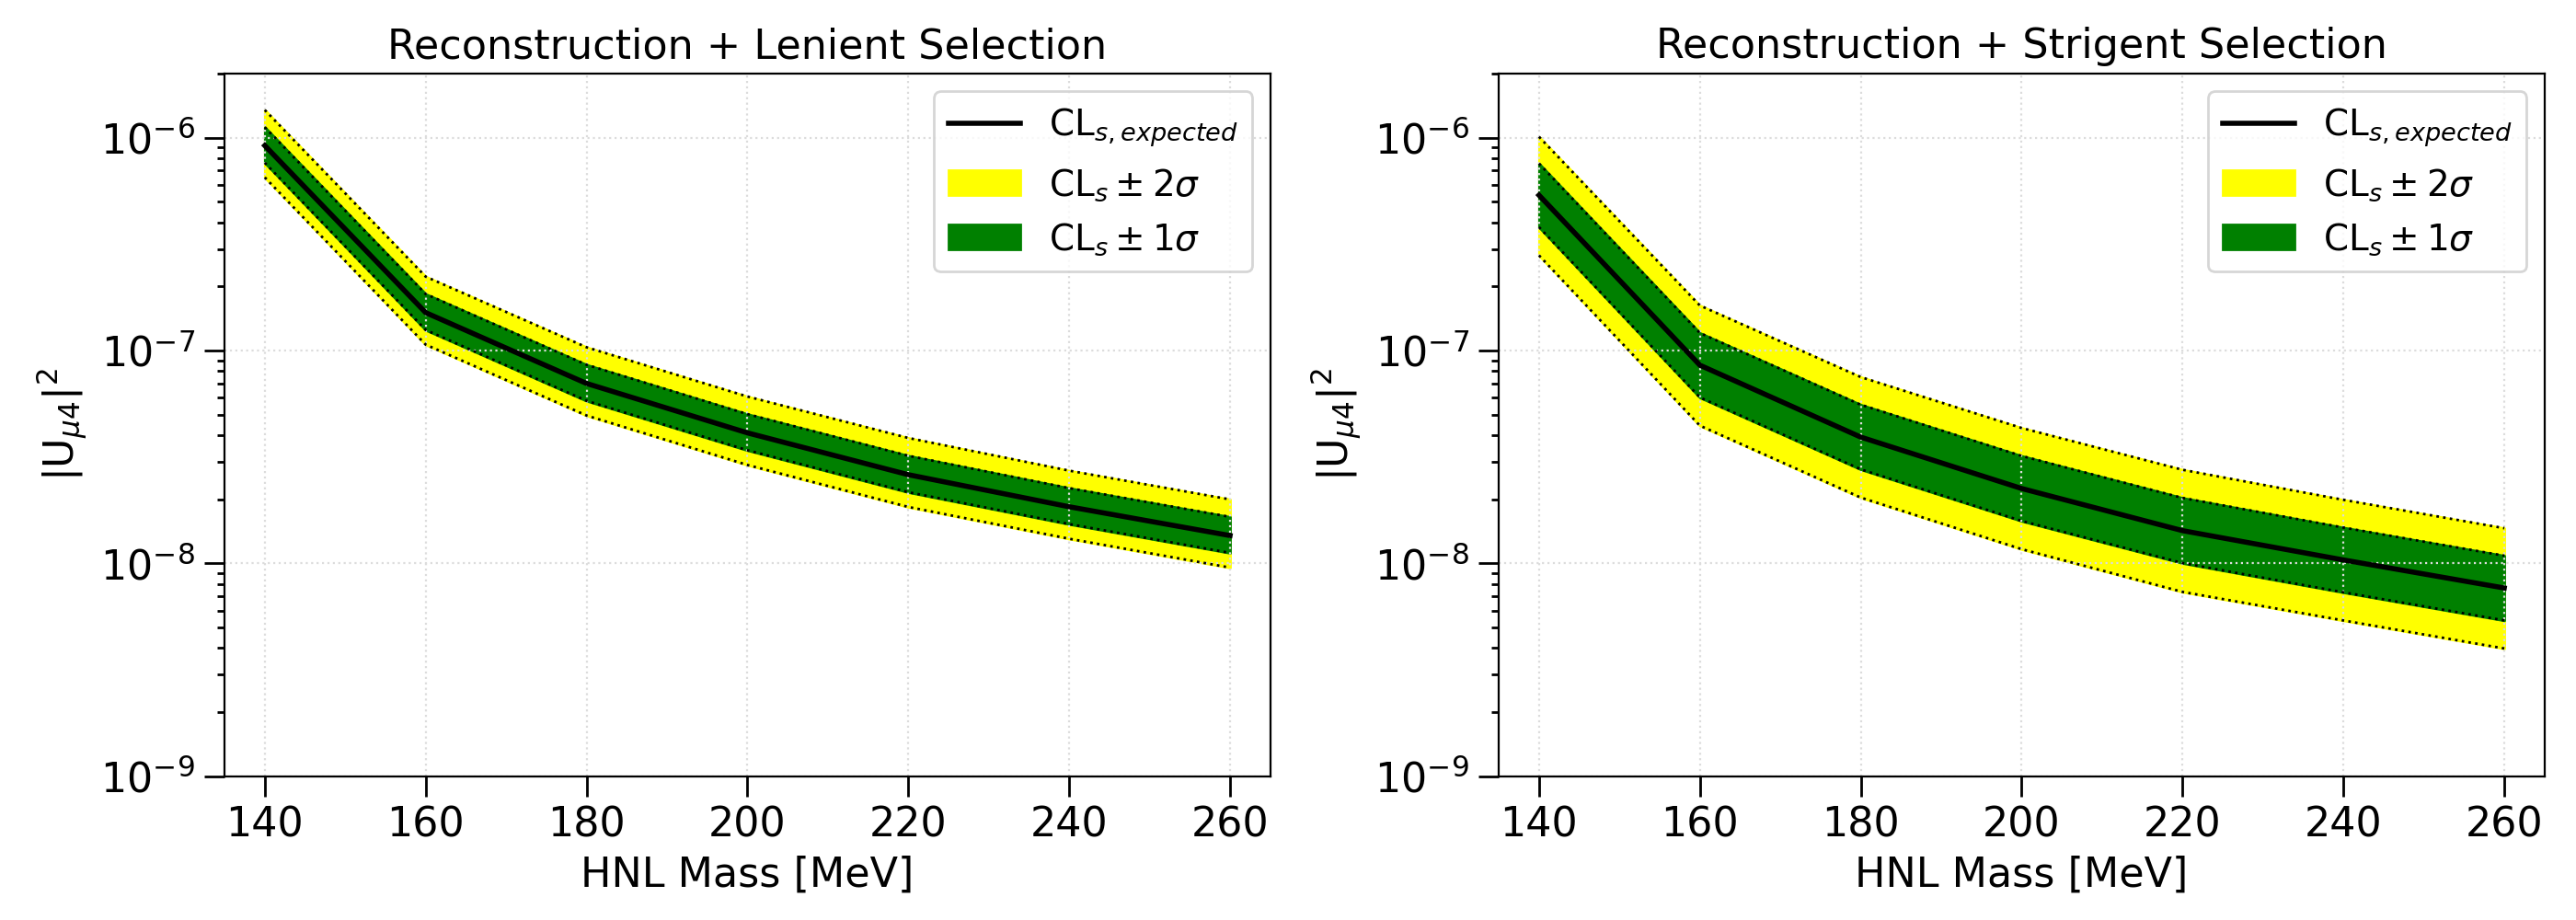
\includegraphics[width=\textwidth]{sensitivity_strict_loose}
    \caption{Expected limits and the Brazil bands on the coupling $|U_{\mu4}|^2$ for Majorana HNLs, for the lenient (left) and stringent distribution (right).}
    \label{fig:nupi0_reco_result}
\vspace{0.5cm}
%\end{figure}
%\begin{figure}[b!]
    \centering
    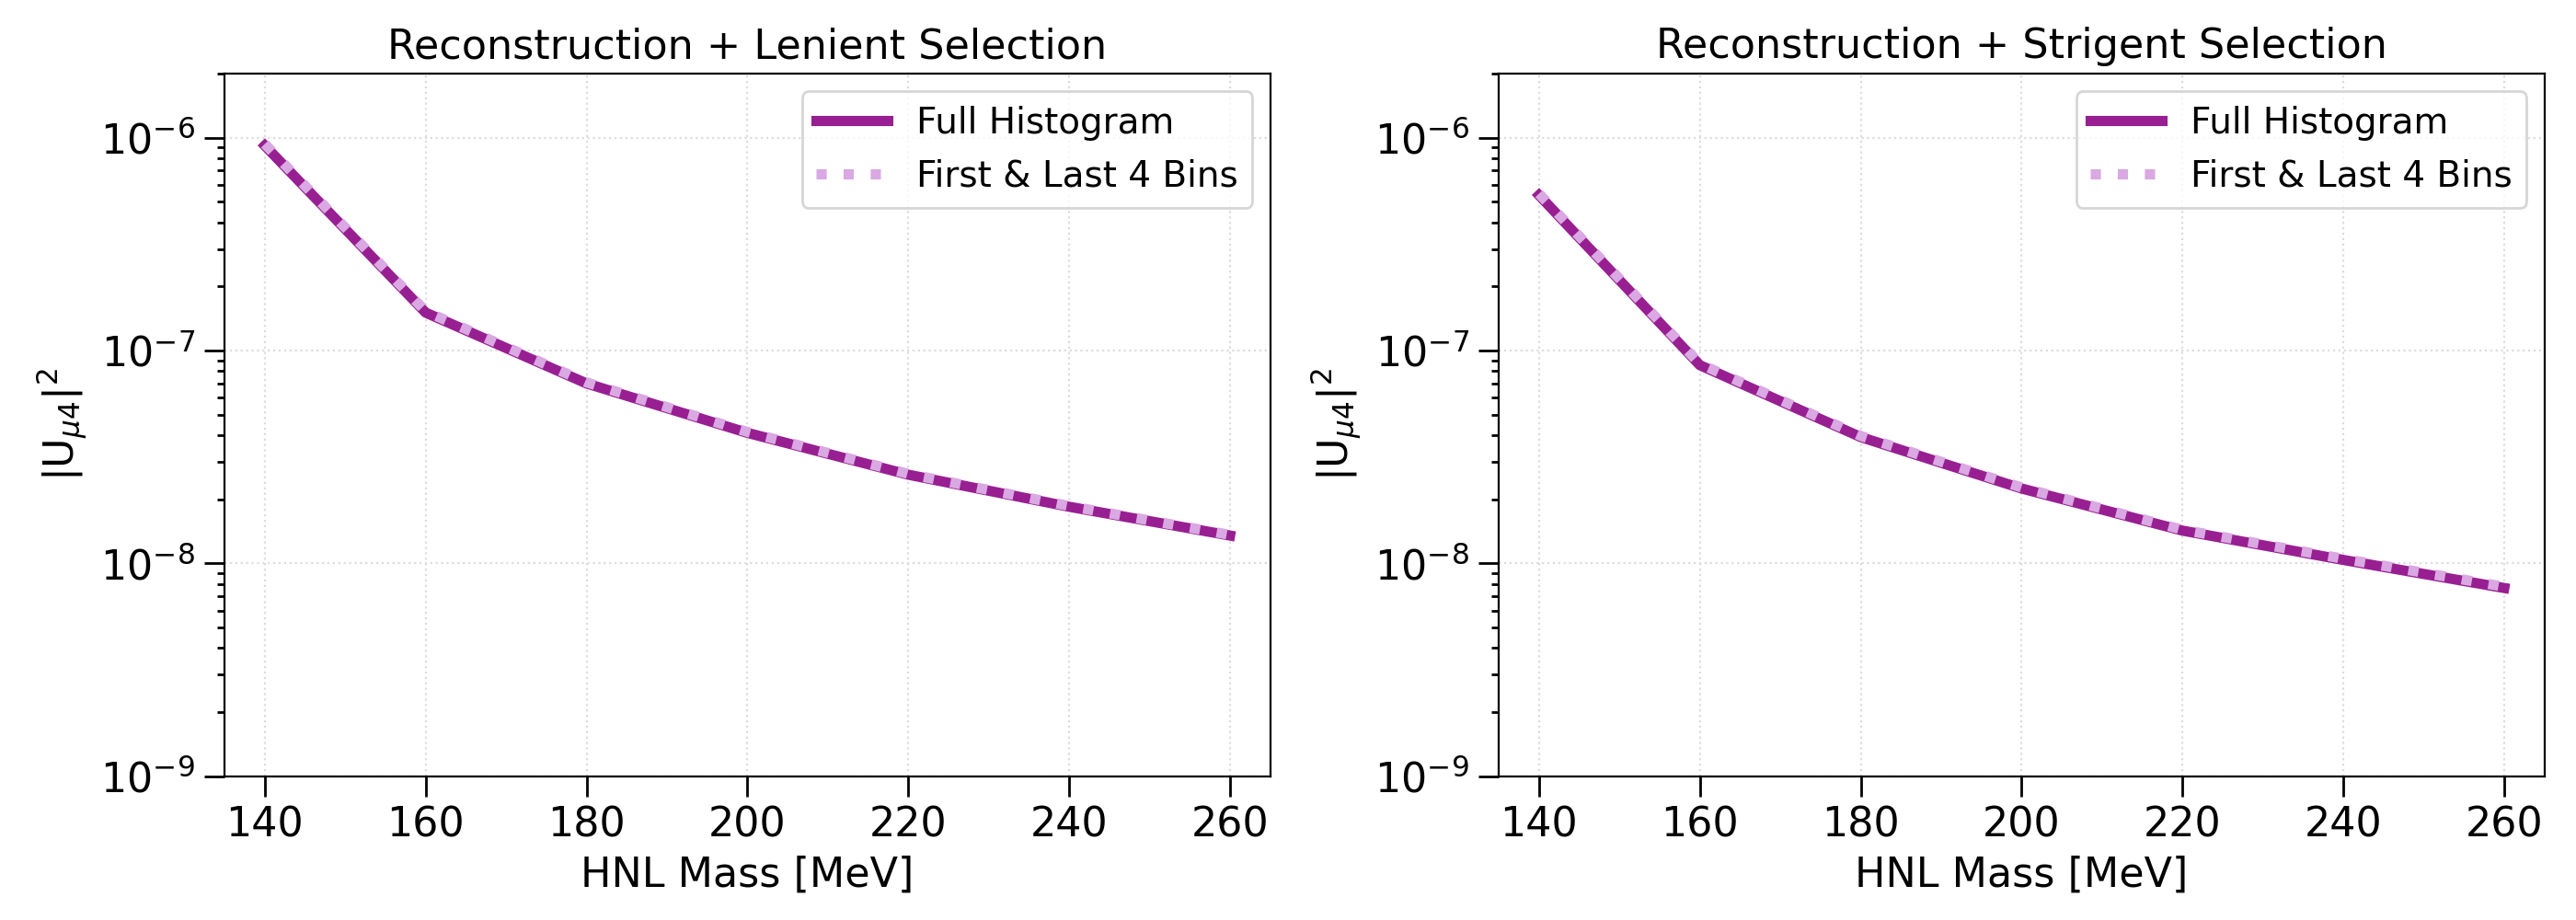
\includegraphics[width=\textwidth]{sensitivity_full_edge}
    \caption{Expected limits on the coupling $|U_{\mu4}|^2$ for Majorana HNLs, comparing between limit setting using the entire histogram or only the edge bins of the lenient (left) and stringent distribution (right).}
    \label{fig:nupi0_reco_full_edge}
\end{figure}

Moreover, Fig. \ref{fig:nupi0_reco_full_edge} shows the comparison between limit setting using the entire histogram and only the first and last 4 bins, which were previously referred to as the timing cut in Chapter \ref{ChapterSelect}. 
The sensitivity limits are the same for both cases.
The result demonstrates that the first and last 4 bins are the highest signal-to-background ratio bins, and therefore are the main contributor to the limits.
This provides a useful insight for future iterations of this analysis indicating the region on the beam bucket distribution should be focused on when performing the selection.
A recommendation is to focus on optimising the signal-to-background only in the edge region.
Another recommendation is to develop different selections for different regions of the bucket, capitalising on their different signal-to-background ratios.

\begin{figure}[b!]
    \centering
    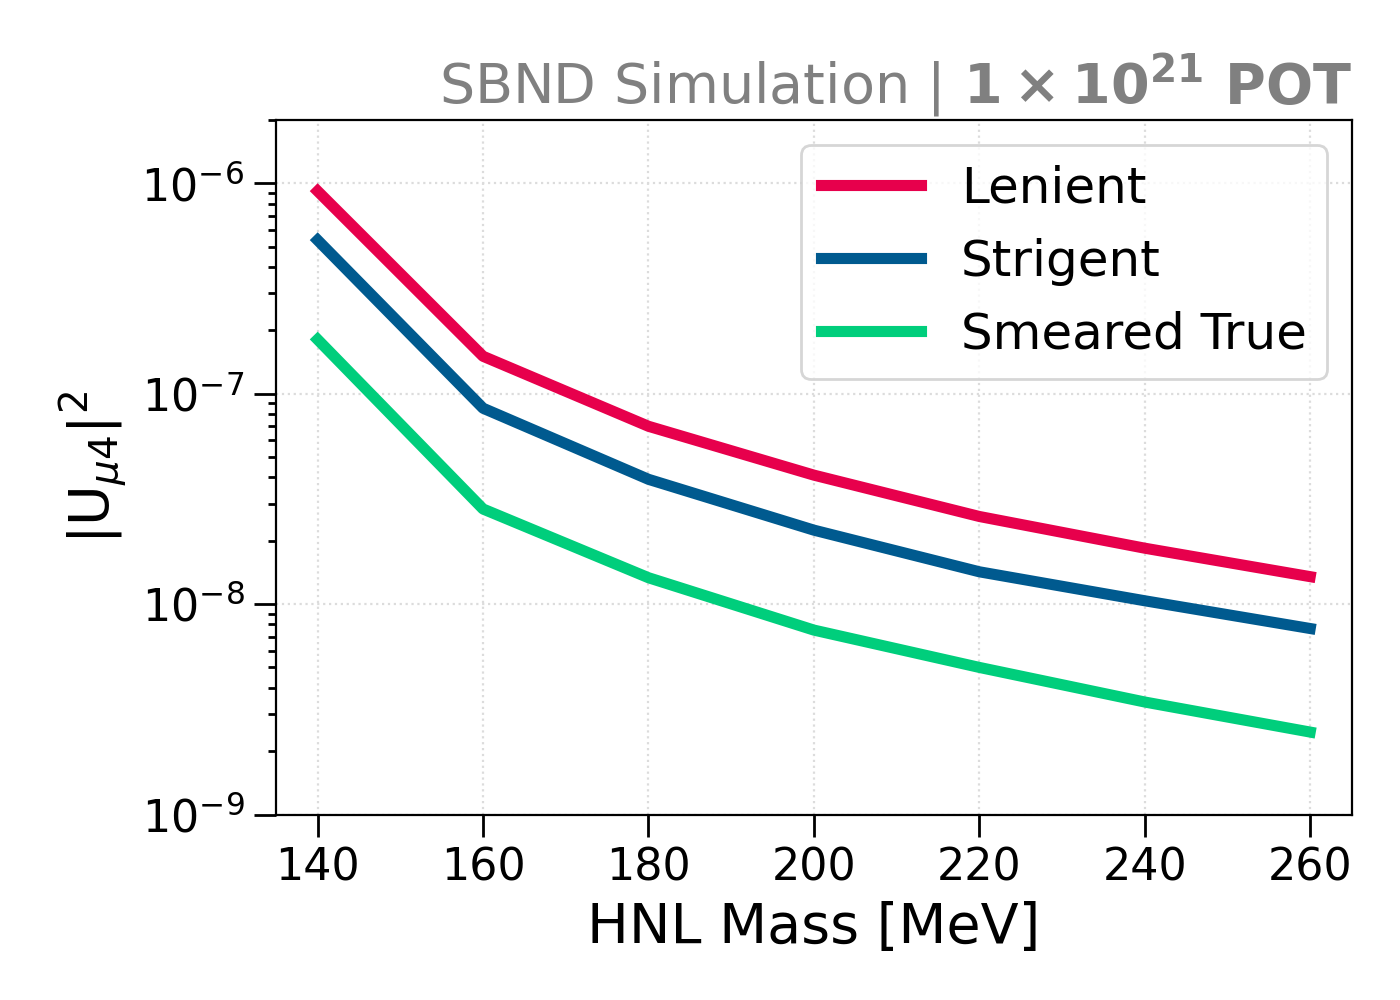
\includegraphics[width=0.7\textwidth]{sensitivity_strict_loose_truth}
    \caption{Expected limits on the coupling $|U_{\mu4}|^2$ for Majorana HNLs, comparing results from the lenient and stringent reconstructed distributions and the smeared truth distribution.}
    \label{fig:nupi0_reco_truth}
\end{figure}

Finally, Fig. \ref{fig:nupi0_reco_truth} shows the upper limits from all three beam bucket distributions.
The result from the smeared truth distribution, as shown by the green line, is significantly more competitive than the results using reconstructed distributions, as shown by the red and blue lines.
The upper limits of the smeared truth distribution range from $1.81 \times 10^{-7}$ to $2.46 \times 10^{-9}$ across the mass range of 140 - 260 MeV. 
As detailed in Section \ref{sec:truth_bucket}, the smeared truth distribution was produced to answer the hypothetical question exploring the impact on sensitivity limits due to timing resolution improvement. 
The background beam bucket distribution of the smeared truth follows a Gaussian with a sigma of 1.73 ns as compared to $1.99$ ns of the reconstructed distribution after the lenient or stringent cut.
The impact of the timing resolution improvement is evident in Fig. \ref{fig:final_truth}, particularly for bins at the edge region.
It can be seen that the background rate is lower while the signal rate is significantly higher in the smeared truth distribution than the reconstructed distribution.
The resulting signal-to-background ratio is therefore higher for the edge bins, driving the sensitivity limits more aggressively. 
%resulting in a higher signal-to-noise ratio
This presents a positive outlook as an area for improvement for SBND to achieve more competitive results in the search for HNLs.
Particularly, this can be done with a more sophisticated timing reconstruction that can resolve the beam bucket with higher resolution $< 2$ ns.

The expected upper limits at 90\% C.L. and the Brazil bands acquired from the three beam bucket distributions are summarised below in Table \ref{table:result}.  

\begin{table}[htbp!]
\begin{center}
	\begin{tabular}{|c| c | c | c | c | c | c|} 
\hline 
& \textbf{Mass [MeV]} & \textbf{Expected Limit} & \textbf{+1$\sigma$} & \textbf{-1$\sigma$} & \textbf{+2$\sigma$} & \textbf{-2$\sigma$}\\

\hline &&&&&& \\[-1.5ex]
\multirow{6}{*}{\rotatebox[origin=c]{90}{\parbox[c]{3.65cm}{\centering \textbf{Lenient} }}} 

& 140 & $9.18\times10^{-7}$ & $1.12\times10^{-6}$ & $7.62\times10^{-7}$ & $1.35\times10^{-6}$ & $6.51\times10^{-7}$ \\
& 160 & $1.51\times10^{-7}$ & $1.84\times10^{-7}$ & $1.25\times10^{-7}$ & $2.22\times10^{-7}$ & $1.07\times10^{-7}$ \\
& 180 & $7.00\times10^{-8}$ & $8.57\times10^{-8}$ & $5.80\times10^{-8}$ & $1.04\times10^{-7}$ & $4.95\times10^{-8}$ \\
& 200 & $4.10\times10^{-8}$ & $5.02\times10^{-8}$ & $3.40\times10^{-8}$ & $6.08\times10^{-8}$ & $2.90\times10^{-8}$ \\
& 220 & $2.61\times10^{-8}$ & $3.20\times10^{-8}$ & $2.16\times10^{-8}$ & $3.88\times10^{-8}$ & $1.84\times10^{-8}$ \\
& 240 & $1.84\times10^{-8}$ & $2.26\times10^{-8}$ & $1.53\times10^{-8}$ & $2.73\times10^{-8}$ & $1.30\times10^{-8}$ \\
& 260 & $1.35\times10^{-8}$ & $1.65\times10^{-8}$ & $1.12\times10^{-8}$ & $2.00\times10^{-8}$ & $9.55\times10^{-9}$ \\ [0.5ex]
\hline &&&&&& \\[-1.5ex]
\multirow{6}{*}{\rotatebox[origin=c]{90}{\parbox[c]{3.65cm}{\centering \textbf{Stringent} }}} 

& 140 & $5.37\times10^{-7}$ & $7.56\times10^{-7}$ & $3.80\times10^{-7}$ & $1.01\times10^{-6}$ & $2.80\times10^{-7}$ \\
& 160 & $8.53\times10^{-8}$ & $1.21\times10^{-7}$ & $6.02\times10^{-8}$ & $1.63\times10^{-7}$ & $4.43\times10^{-8}$ \\
& 180 & $3.92\times10^{-8}$ & $5.56\times10^{-8}$ & $2.76\times10^{-8}$ & $7.50\times10^{-8}$ & $2.04\times10^{-8}$ \\
& 200 & $2.25\times10^{-8}$ & $3.20\times10^{-8}$ & $1.58\times10^{-8}$ & $4.32\times10^{-8}$ & $1.17\times10^{-8}$ \\
& 220 & $1.42\times10^{-8}$ & $2.03\times10^{-8}$ & $1.00\times10^{-8}$ & $2.75\times10^{-8}$ & $7.34\times10^{-9}$ \\
& 240 & $1.04\times10^{-8}$ & $1.47\times10^{-8}$ & $7.31\times10^{-9}$ & $1.99\times10^{-8}$ & $5.39\times10^{-9}$ \\
& 260 & $7.65\times10^{-9}$ & $1.09\times10^{-8}$ & $5.39\times10^{-9}$ & $1.46\times10^{-8}$ & $3.98\times10^{-9}$ \\ [0.5ex]
\hline &&&&&& \\[-1.5ex]
\multirow{6}{*}{\rotatebox[origin=c]{90}{\parbox[c]{3.65cm}{\centering \textbf{Smeared Truth} }}} 

& 140 & $1.81\times10^{-7}$ & $2.45\times10^{-7}$ & $1.35\times10^{-7}$ & $3.21\times10^{-7}$ & $1.05\times10^{-7}$ \\
& 160 & $2.83\times10^{-8}$ & $3.84\times10^{-8}$ & $2.11\times10^{-8}$ & $5.05\times10^{-8}$ & $1.63\times10^{-8}$ \\
& 180 & $1.33\times10^{-8}$ & $1.81\times10^{-8}$ & $9.94\times10^{-9}$ & $2.38\times10^{-8}$ & $7.70\times10^{-9}$ \\
& 200 & $7.52\times10^{-9}$ & $1.02\times10^{-8}$ & $5.62\times10^{-9}$ & $1.34\times10^{-8}$ & $4.38\times10^{-9}$ \\
& 220 & $5.00\times10^{-9}$ & $6.78\times10^{-9}$ & $3.73\times10^{-9}$ & $8.90\times10^{-9}$ & $2.90\times10^{-9}$ \\
& 240 & $3.42\times10^{-9}$ & $4.65\times10^{-9}$ & $2.55\times10^{-9}$ & $6.10\times10^{-9}$ & $1.99\times10^{-9}$ \\
& 260 & $2.46\times10^{-9}$ & $3.34\times10^{-9}$ & $1.84\times10^{-9}$ & $4.39\times10^{-9}$ & $1.44\times10^{-9}$ \\ [0.5ex]
\hline
\end{tabular}
\end{center}
\caption{Table summarising results of the limits on the coupling $|U_{\mu4}|^2$.}
\label{table:result}
\end{table}

\subsection{Comparison With Other Experiments}

Fig. \ref{fig:sensitivity} shows the expected upper limits of SBND on the coupling $|U_{\mu4}|^2$ of Majorana HNLs, comparing against existing experimental results that were previously discussed in Section \ref{sec2Previous}.
All limits presented here are at 90\% C.L.

For the limits acquired from the lenient and stringent distributions, as shown by the solid red and blue line respectively, they are comparable to existing limits.
The lenient limit is almost the same as the limit achieved by the MicroBooNE experiment, as shown by the solid light blue line.
On the other hand, the stringent limit is slightly more competitive than MicroBooNe, excluding a new region of the coupling in the mass range $< 200$ MeV.
However, in the mass range $> 200$ MeV, the phase space is already excluded by the E949 and NA62 experiments, as shown by the dashed pink and orange lines.
These two limits feature the first benchmark of SBND in this phase space of HNLs, given the current detector and reconstruction capabilities.

\begin{figure}[bp!]
    \centering
    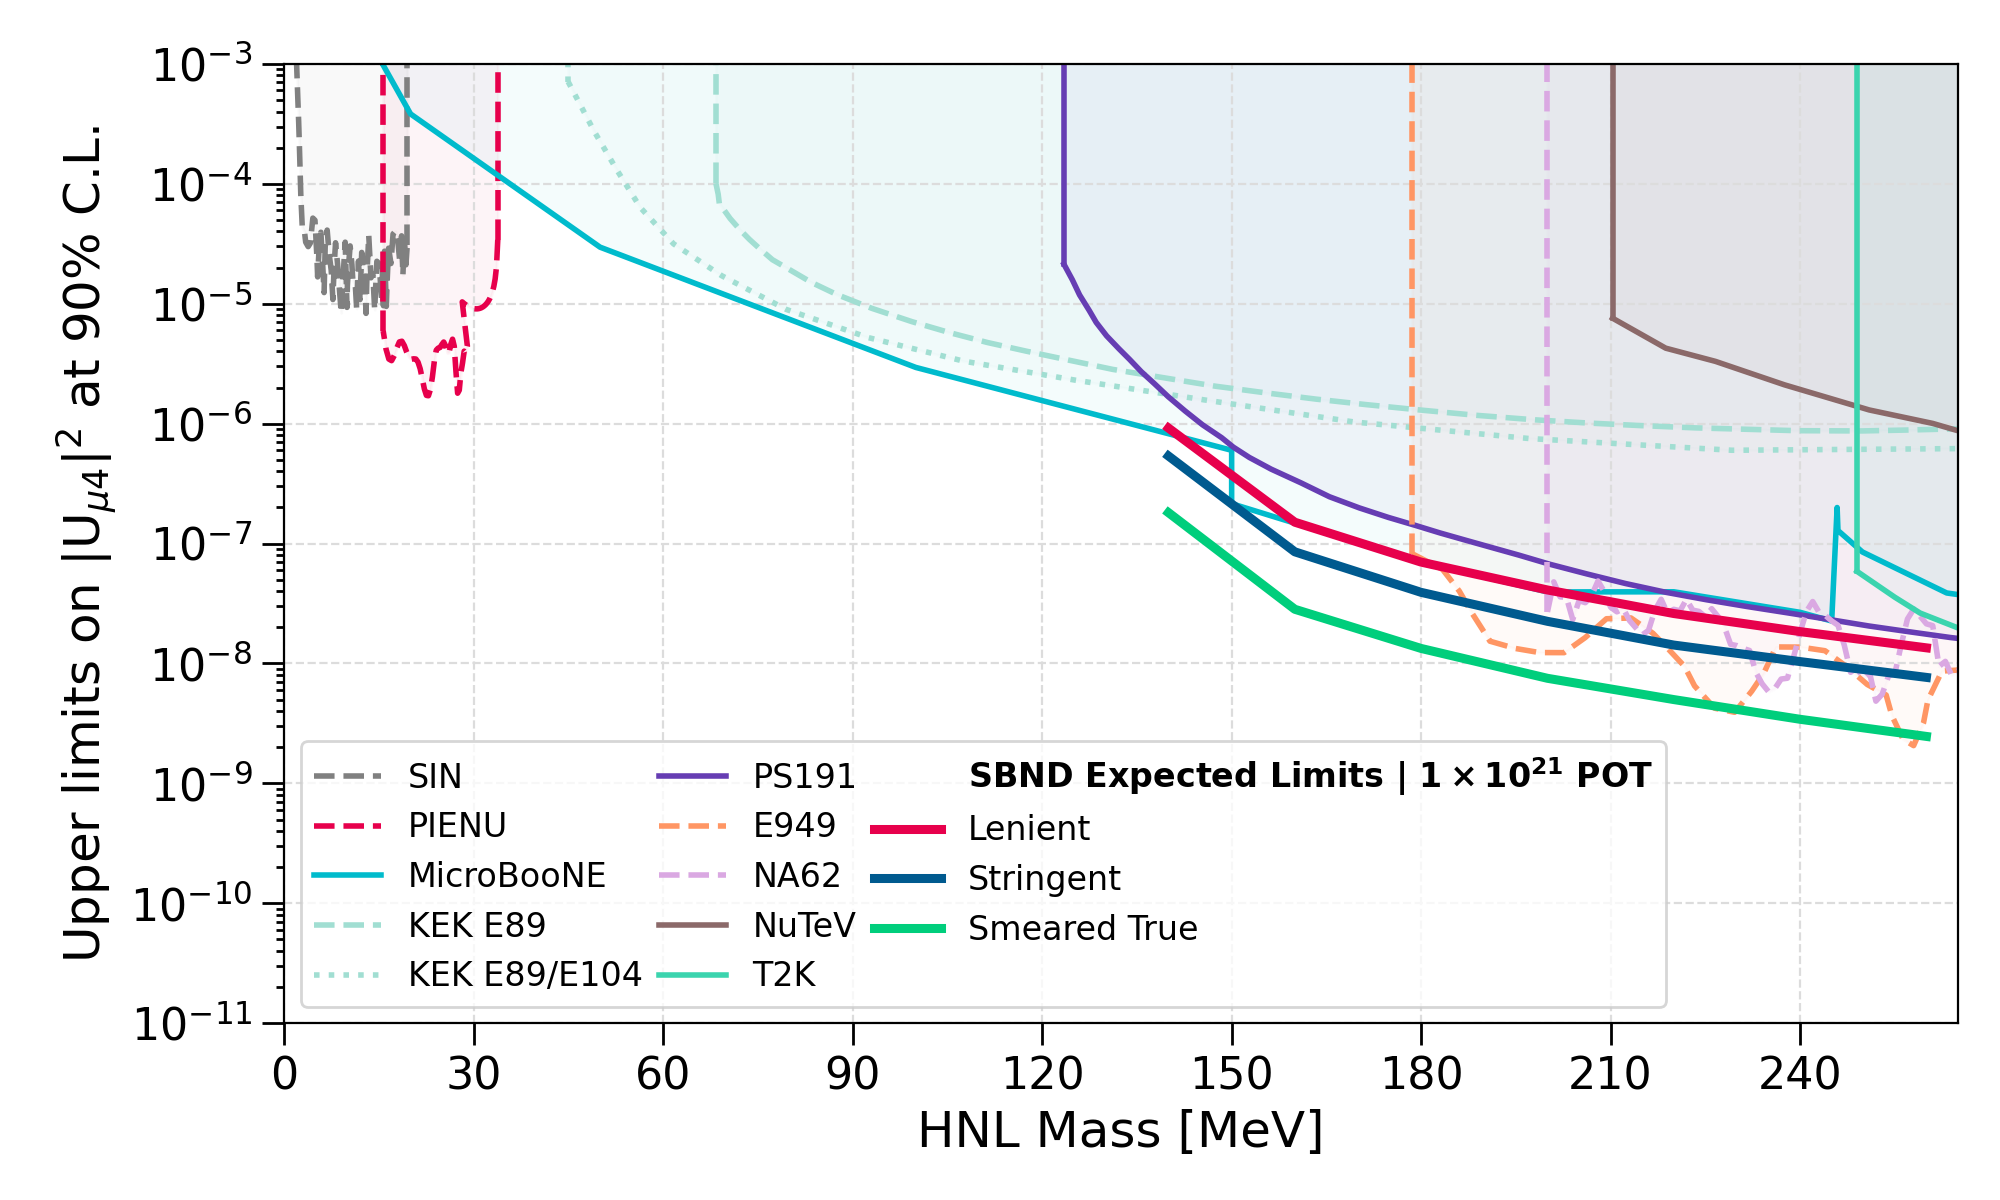
\includegraphics[width=\textwidth]{sensitivity}
    \caption{Sensitivity contour of the upper limits on the coupling $|U_{\mu4}|^2$ for Majorana HNLs within the mass range of $0 < m_N < 265$ MeV, comparing the expected result from SBND against existing experimental results.}
    \label{fig:sensitivity}
\end{figure}

The limit acquired from the smeared truth distribution, as shown by the green line, is the most competitive out of the three results presented here.
The result is projected to exclude a new region beyond the existing limits from the MicroBooNE, E949 and NA62 experiments.
This demonstrates the potential of the physics capability of SBND, under the assumption of an exposure of $1 \times 10^{21}$ POT and an exceptional timing reconstruction with a resolution of 1.73 ns.
The POT exposure presented here is equivalent to 3 years of physics data taking, which allows for a lot of time and opportunities to work on improving the timing reconstruction of SBND to achieve the target resolution from the time of writing.

%********************************** %First Section  **************************************
\section{Concluding Remarks}
\label{sec:result_remarks}

Three limits on the coupling $|U_{\mu4}|^2$ of Majorana HNLs are presented in this chapter to demonstrate the range of the physics capability of SBND.
The limits from the lenient and stringent beam bucket distribution demonstrate the current performance of SBND, which is currently comparable to existing experimental limits.
The limit from the smeared truth distribution is the most competitive that can exclude a new region not yet explored by other experiments.
This limit also demonstrates the potential that SBND can achieve if the timing reconstruction is improved with a better timing resolution.
Although ambitious, this goal is within reach in the next couple of years given the ongoing work towards a nanosecond timing resolution at SBND, one of which was presented in Chapter \ref{ChapterDAQ} and many more to be expected in the near future.
 


